%!TEX root = ../main.tex
For the analysis of our algorithms and data structures, we decided to analyze the run time on two types of instances, one with a fixed number of vertices ($|V|=1000$) and a density of edges ranging from 5 to 100\% and an other one with a density of edges fixed (10\%) and a number of vertices varying from $|V|=1000$ to $|V|=5000$. For all our instances, the maximum capacity of an edge is 10000.
Each algorithm has been tested with each data structure.

\section{Instances generation}
To obtain the necessary instances, we implement instances generators which respects the characteristics of the network graphs (a connected graph where each vertex has at least one incoming and one outgoing edge). \\

For the density variation instances, we first create a minimal connected graph. To do this, let $Connected$ be the set of the connected vertices, $DoubleConnected$ the set of vertex having at least one incoming and one outgoing edge, $Edges$ the set of edges and $AllEdges$ the set of all possible edges. Initially, $Connected$ contains the vertex 0, $DoubleConnected$ and $Edges$ are empty and $AllEdges$ contains all possible edges. When we want to add a vertex $v$ to the graph, we take a random vertex $r$ from $Connected$, add the edge ($v$,$r$) in $Edges$, add $v$ in $Connected$, remove the edges ($v$,$r$) and ($r$,$v$) from $AllEdges$ and add $r$ in $DoubleConnected$. After adding our 1000 vertices, we have a connected graph where each vertex has one incoming edge and sometimes at least one outgoing edge (all vertices in $DoubleConnected$).

For each vertex not present in $DoubleConnected$, we take a random vertex from $Connected$, add the edge between them in $Edges$ and remove this edge and its opposite from $AllEdges$. For this step, to avoid adding an edge (or its opposite) which is already present in the graph, we check if the new edge and its opposite are not present in $Edges$. We thus have a connected graph where each vertex has one incoming edge and at least one outgoing edge.

We then add the necessary number of edges to obtain the desired density. We take a random edge from $AllEdges$, add it to $Edges$ and remove it and its opposite from $AllEdges$. A first graph is generated when we have a density of 5\%. We add it edges to obtain a density of 10\% and generate a second graph. And so on up to 100\%. At the end, a density variation instance is composed by twenty graphs where each graph generated before an other one is a sub-graph of the latter.

With $|V|=1000$, a complete graph has $\frac{(|V|-1)(|V|)}{2} = 499500$ edges.\\

For the size variation instances, we use the same technique as for the density variation instances without the $AllEdges$ set. Indeed, it is not necessary to generate all possible edges for graphs with a 10\% of edge density. Especially when we know that a complete graph with $|V|=5000$ has 12497500 edges. To know if an edge (or its opposite) is already present in the graph, we check if it is contained in $Edges$.

We generate a network graph with $|V|=1000$ and an edge density of 10\%. We add it 500 vertices and the corresponding edges to respect the characteristics of the network graphs. We add then the necessary edges to keep a 10\% edge density and generate this new graph. And so on until $|V|=5000$. At the end, a size variation instance is composed by ten graphs where each graph generated before an other one is a sub-graph of the latter. \\

For our tests, we generate 10 instances of each type.

\section{Best Push-Relabel heuristics}
We have 3 variants of the Push-Relabel algorithm with different complexities so we compare their run time to select the one with the best performance. We did the comparison for our 2 type of instances.

\subsection{Density variation instances}
The Figure~\ref{fig:PRs} represents the average run time of the 3 variants of Push-Relabel on all instances. As we can see, the generic Push-Relabel offers the best results.

%TODO on essaye d'expliquer pourquoi ou tout ce qui est explication, on le fait dans la partie analyse?

\begin{figure}[H]
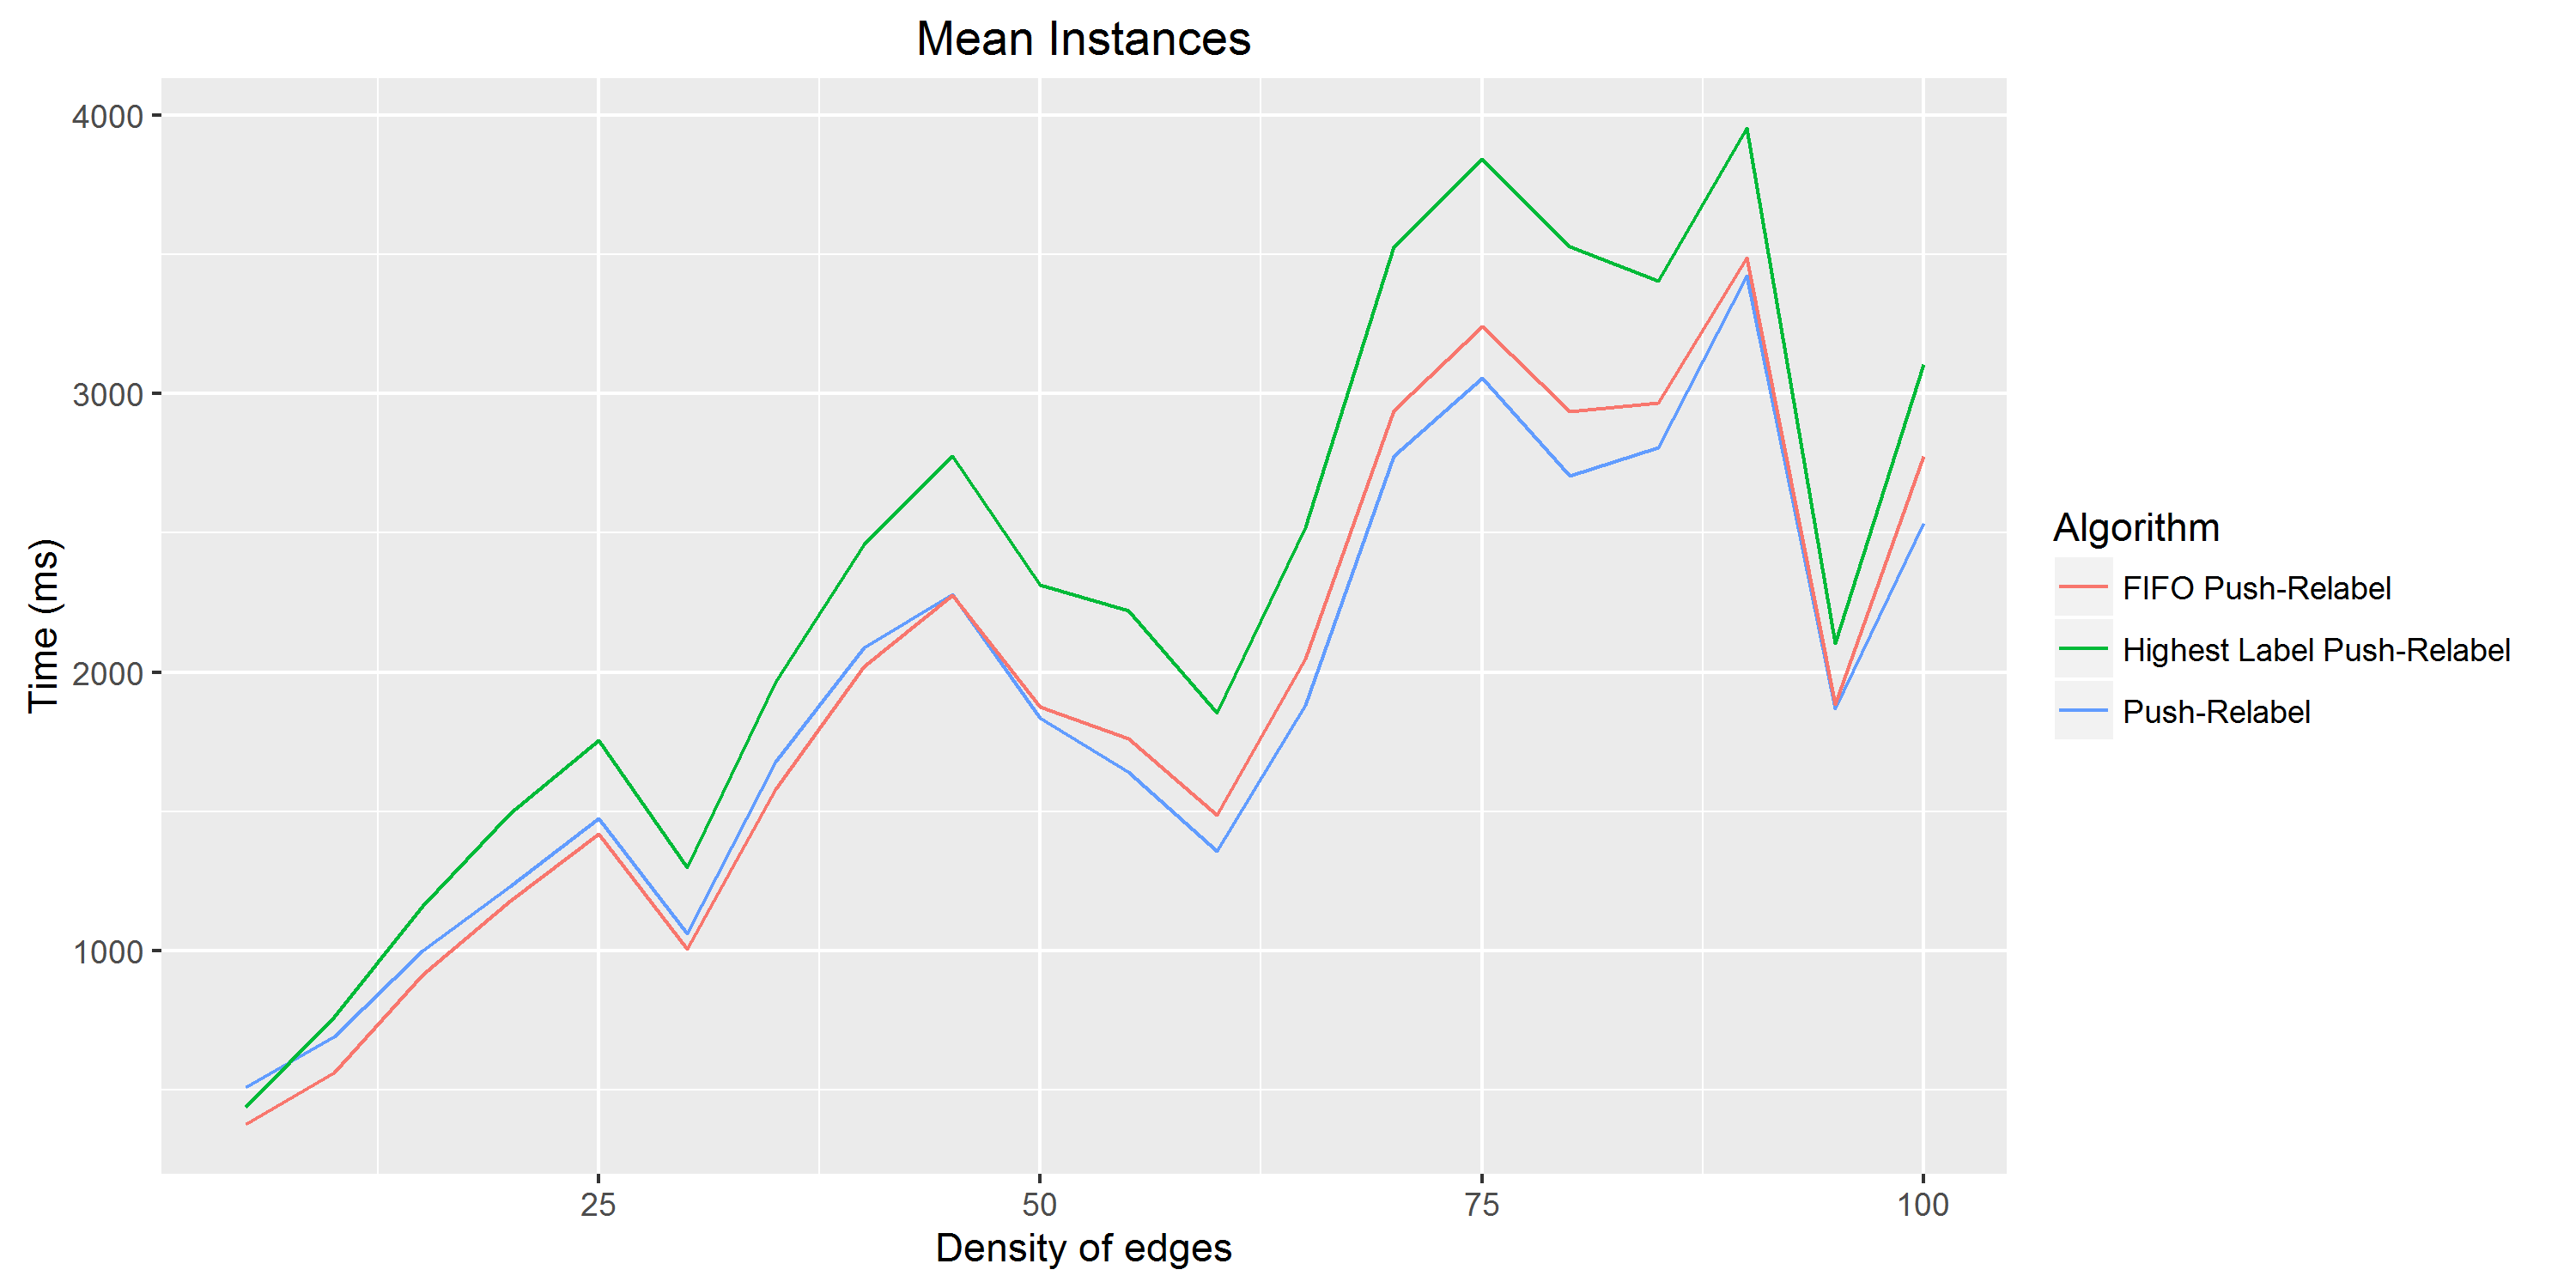
\includegraphics[scale=0.65]{images/meanPRs.png}
\caption{Average run time on all instances for three variants of Push-Relabel.}
\label{fig:PRs}
\end{figure}

\subsection{Size variation instances}
Pas encore fait mais suspense, qui va gagner? HLPR, FPR ou le redoutable PR?

\section{Results}
To obtain the run time of an algorithm with a defined data structure on a specific instance, we make the average of 10 executions	. To be certain of the accuracy of our results, we execute 5 times the same tests in order to study the variance of the run time. The run time varied, on average, by 1\%. We therefore consider that our results are relevant.

\subsection{Density variation instances}
We tested on the 10 density variation instances, Edmonds-Karp, Ford-Fulkerson with scaling and Push-Relabel with our 5 data structures. The entire results can be found in the appendix but here is the most interesting ones.

\subsubsection{Edmonds-Karp}
The Figure~\ref{fig:EK1} represents the run time of Edmonds-Karp with all data structures on the instance 1. As we can see, the data structures based on the sparse set are better than the other one. The hash map and tree map are the least efficient. These observations are the same for all instances. We can conclude that the most appropriate data structure for Edmonds-Karp is the Split Array.

\begin{figure}[H]
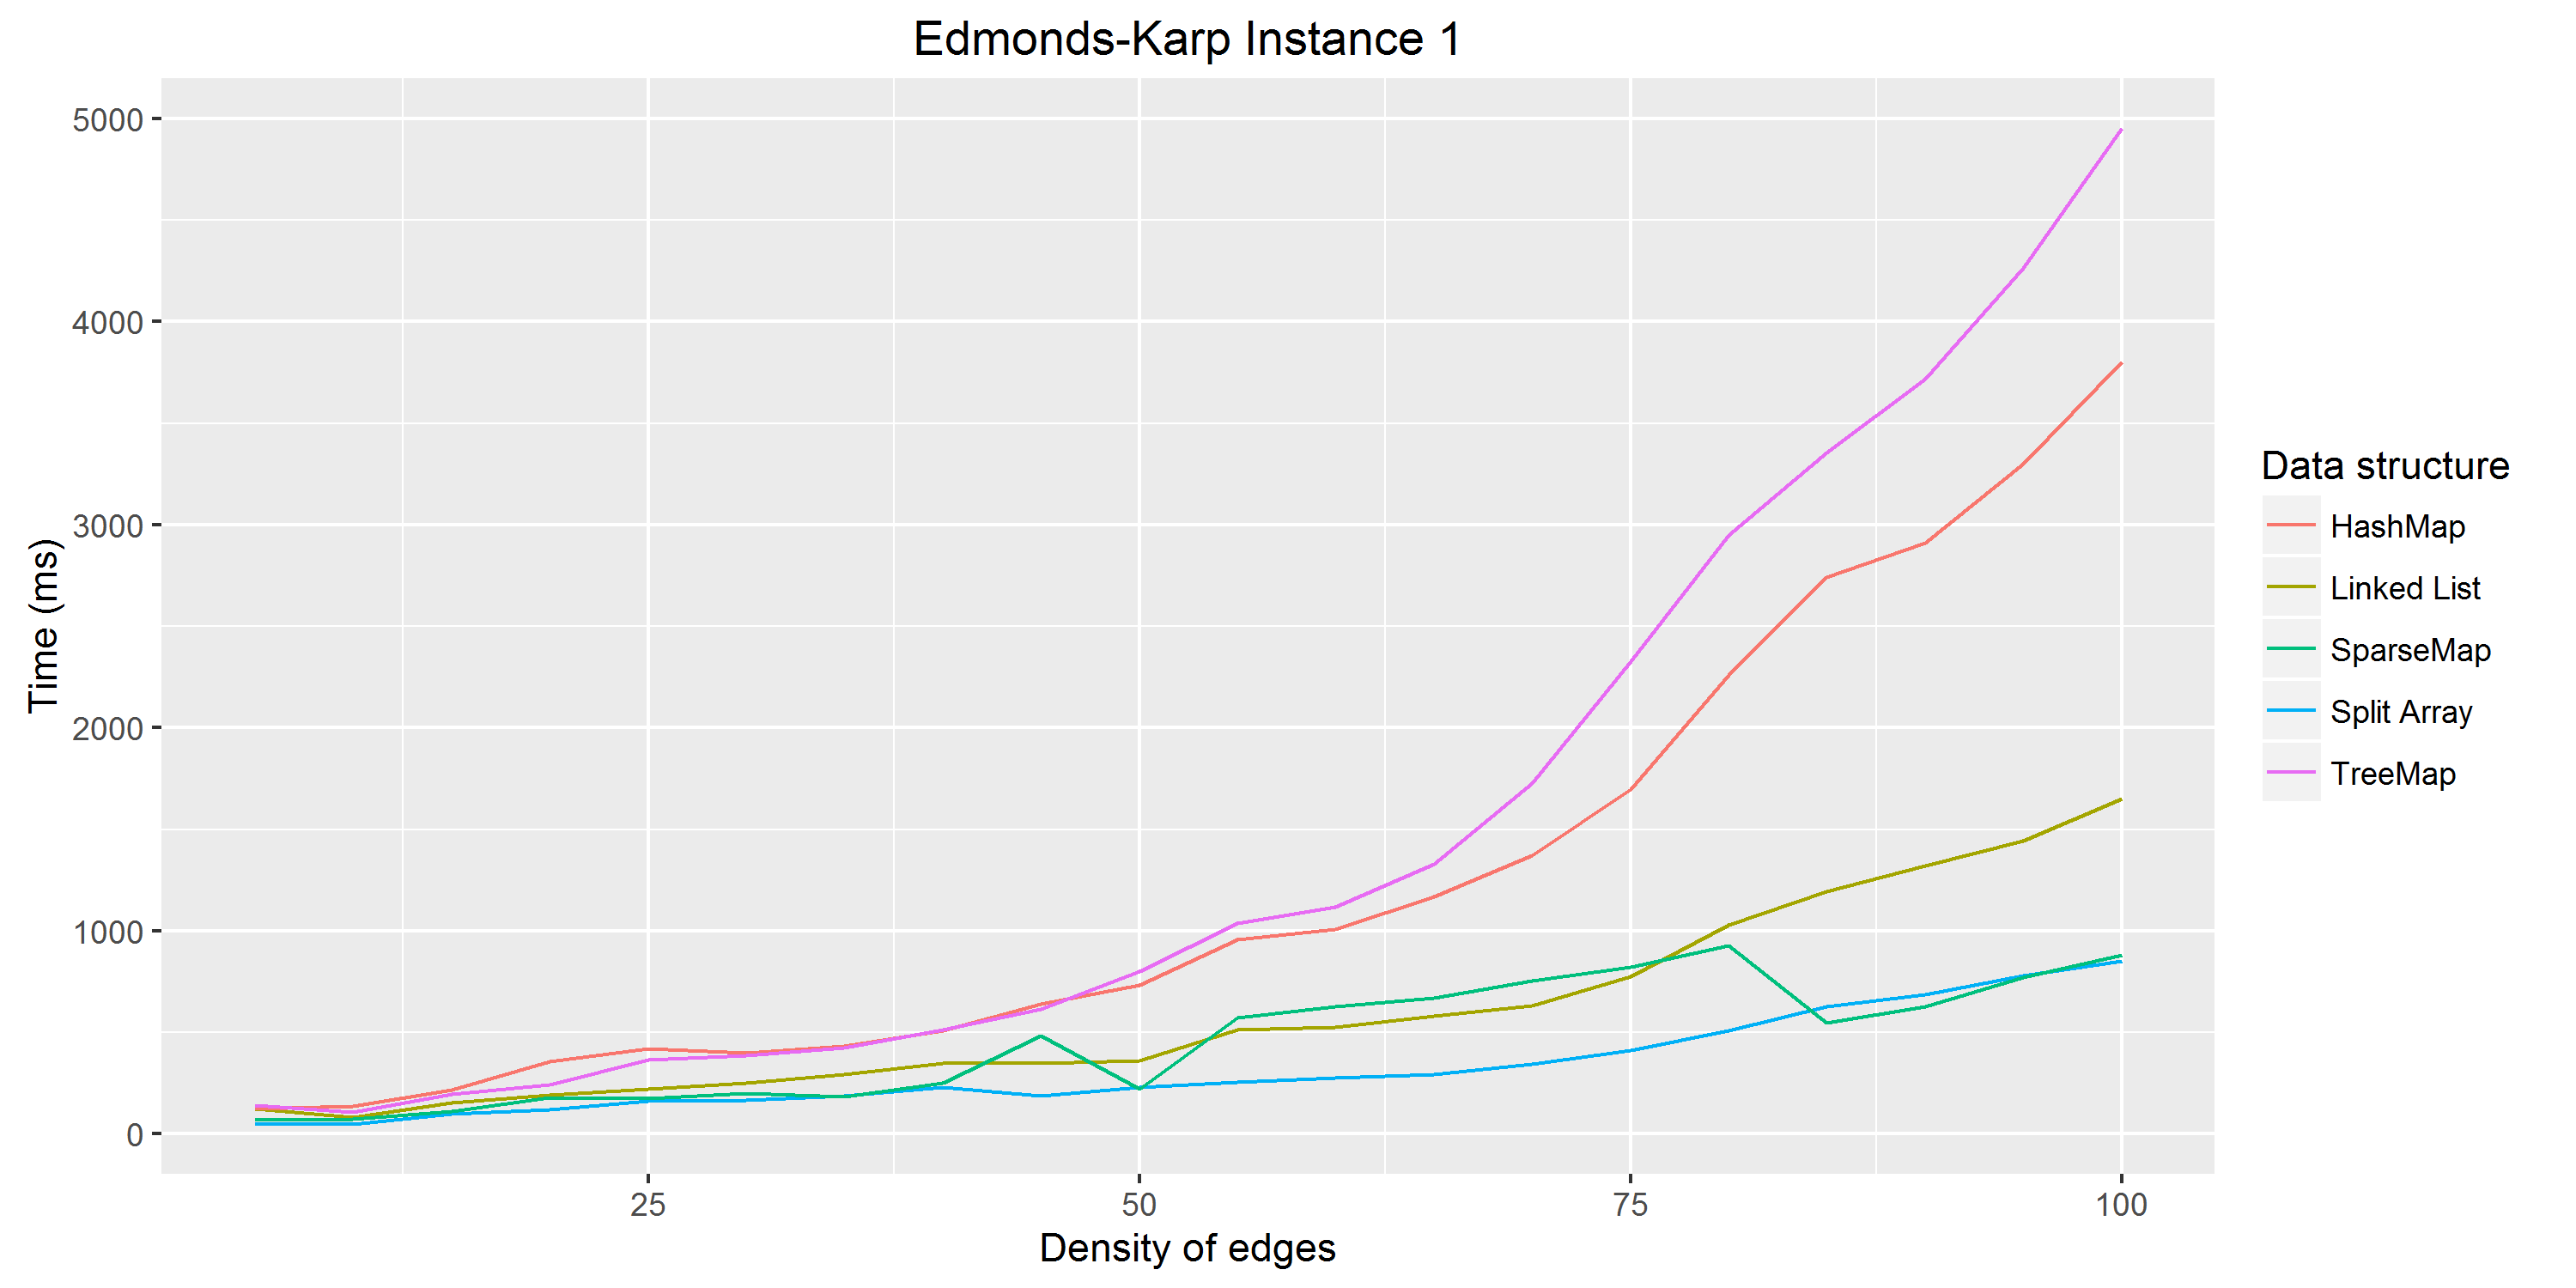
\includegraphics[scale=0.63]{images/EK1.png}
\caption{Run time of Edmonds-Karp on the instance 1.}
\label{fig:EK1}
\end{figure}

One of the most blatant observations on Edmonds-Karp is that it is very regular, what we can observe in the Figure~\ref{fig:EKmean}, which represents the run time on each instance, with its best data structure, the Split Array. Indeed, Edmonds-Karp solve the maximum flow problem on complete graphs with $|V|=1000$ with a run time ranging from 750 to 1000 ms.

\begin{figure}[H]
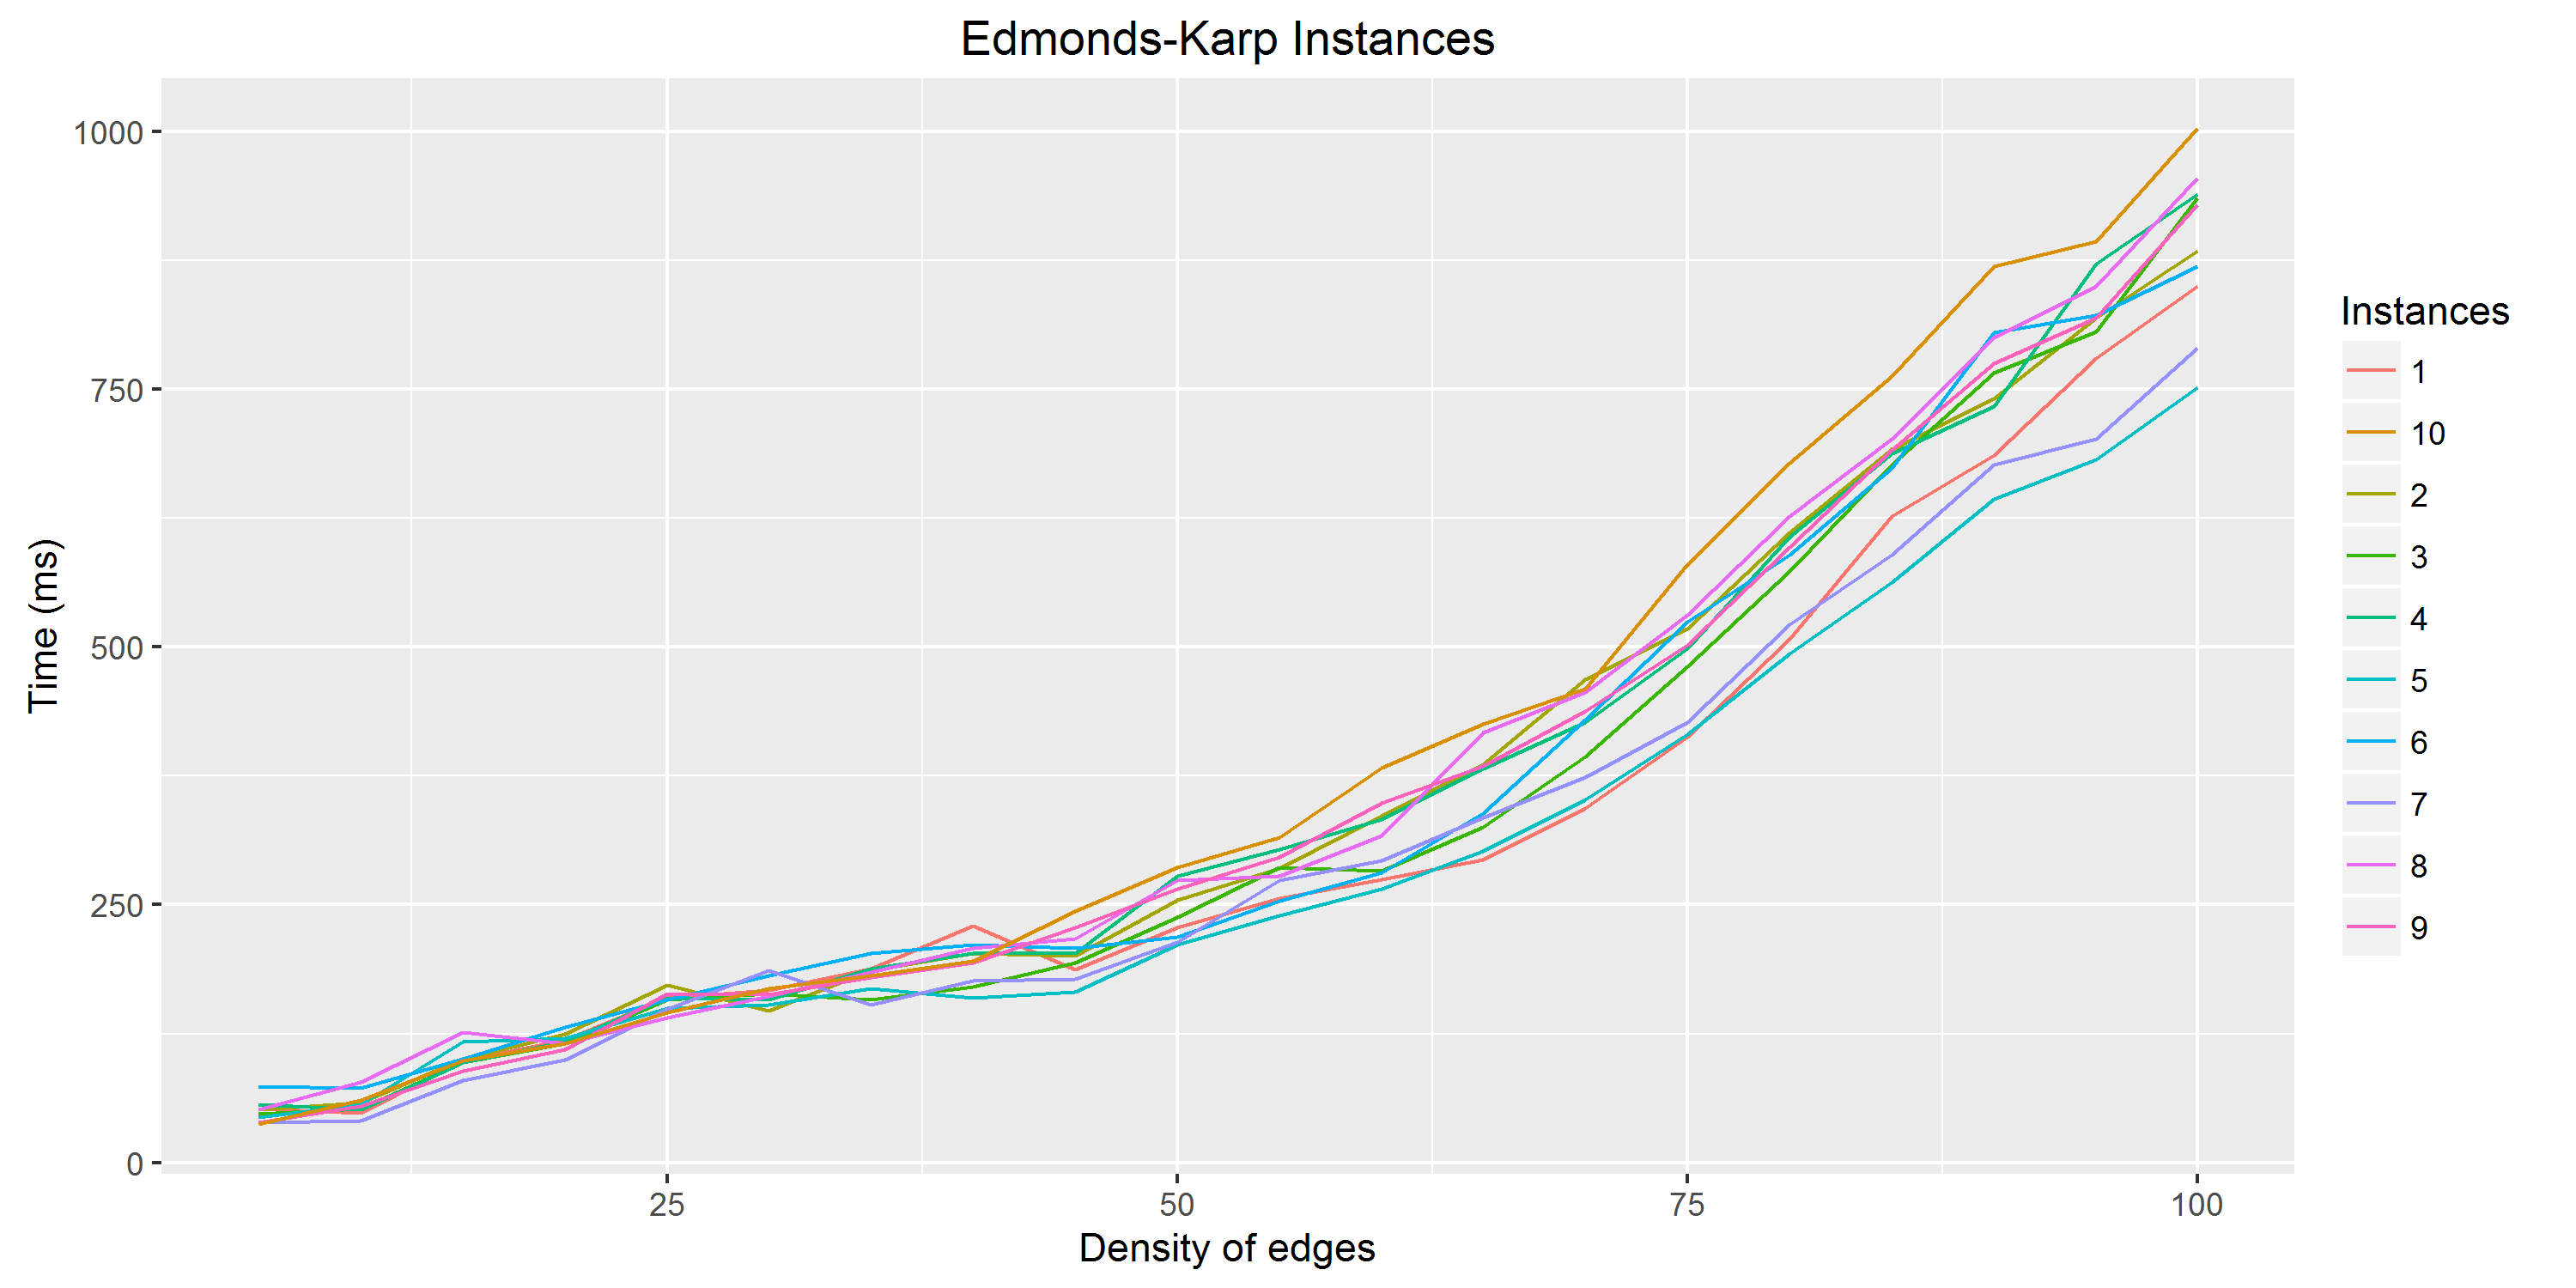
\includegraphics[scale=0.63]{images/EKmean.png}
\caption{Run time of Edmonds-Karp on all instances.}
\label{fig:EKmean}
\end{figure}

\subsubsection{Ford-Fulkerson with scaling}
The Figure~\ref{fig:FF2} and the Figure~\ref{fig:FF6} represent well the behaviour of Ford-Fulkerson with scaling. Sometimes regular, sometimes less, it remains stable. As we can see, the Linked List provides poor performance while the SparseMap seems to be the most appropriate data structure for Ford-Fulkerson with scaling.

\begin{figure}[H]
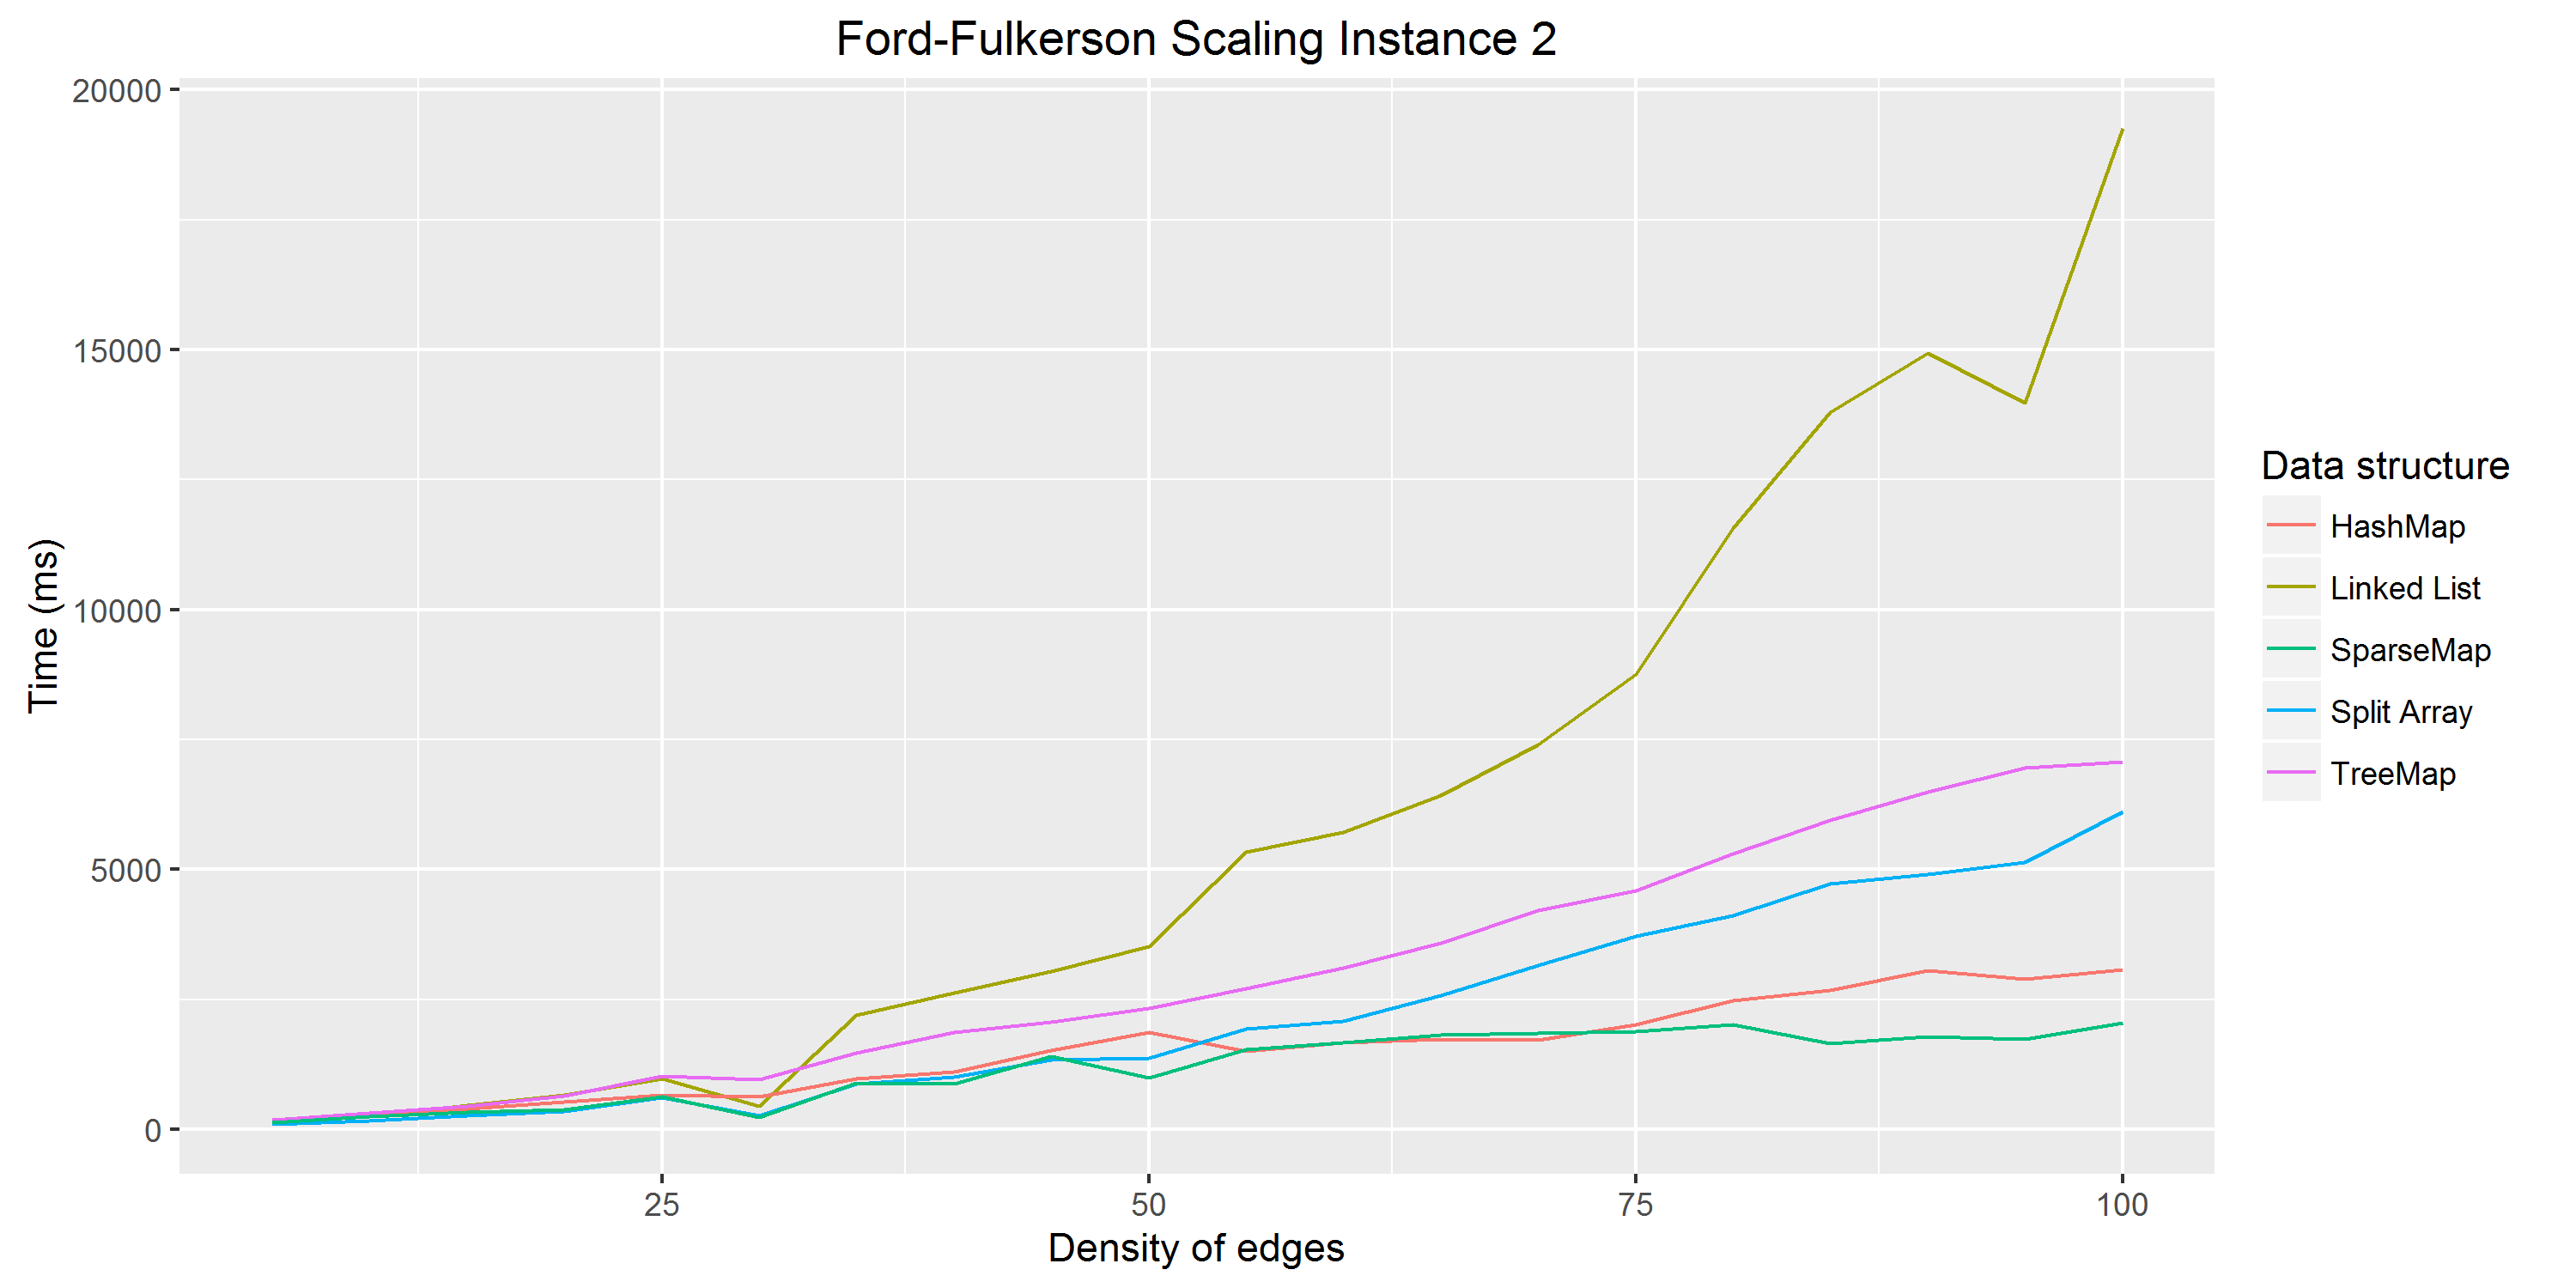
\includegraphics[scale=0.63]{images/FF2.png}
\caption{Run time of Ford-Fulkerson scaling on the instance 2.}
\label{fig:FF2}
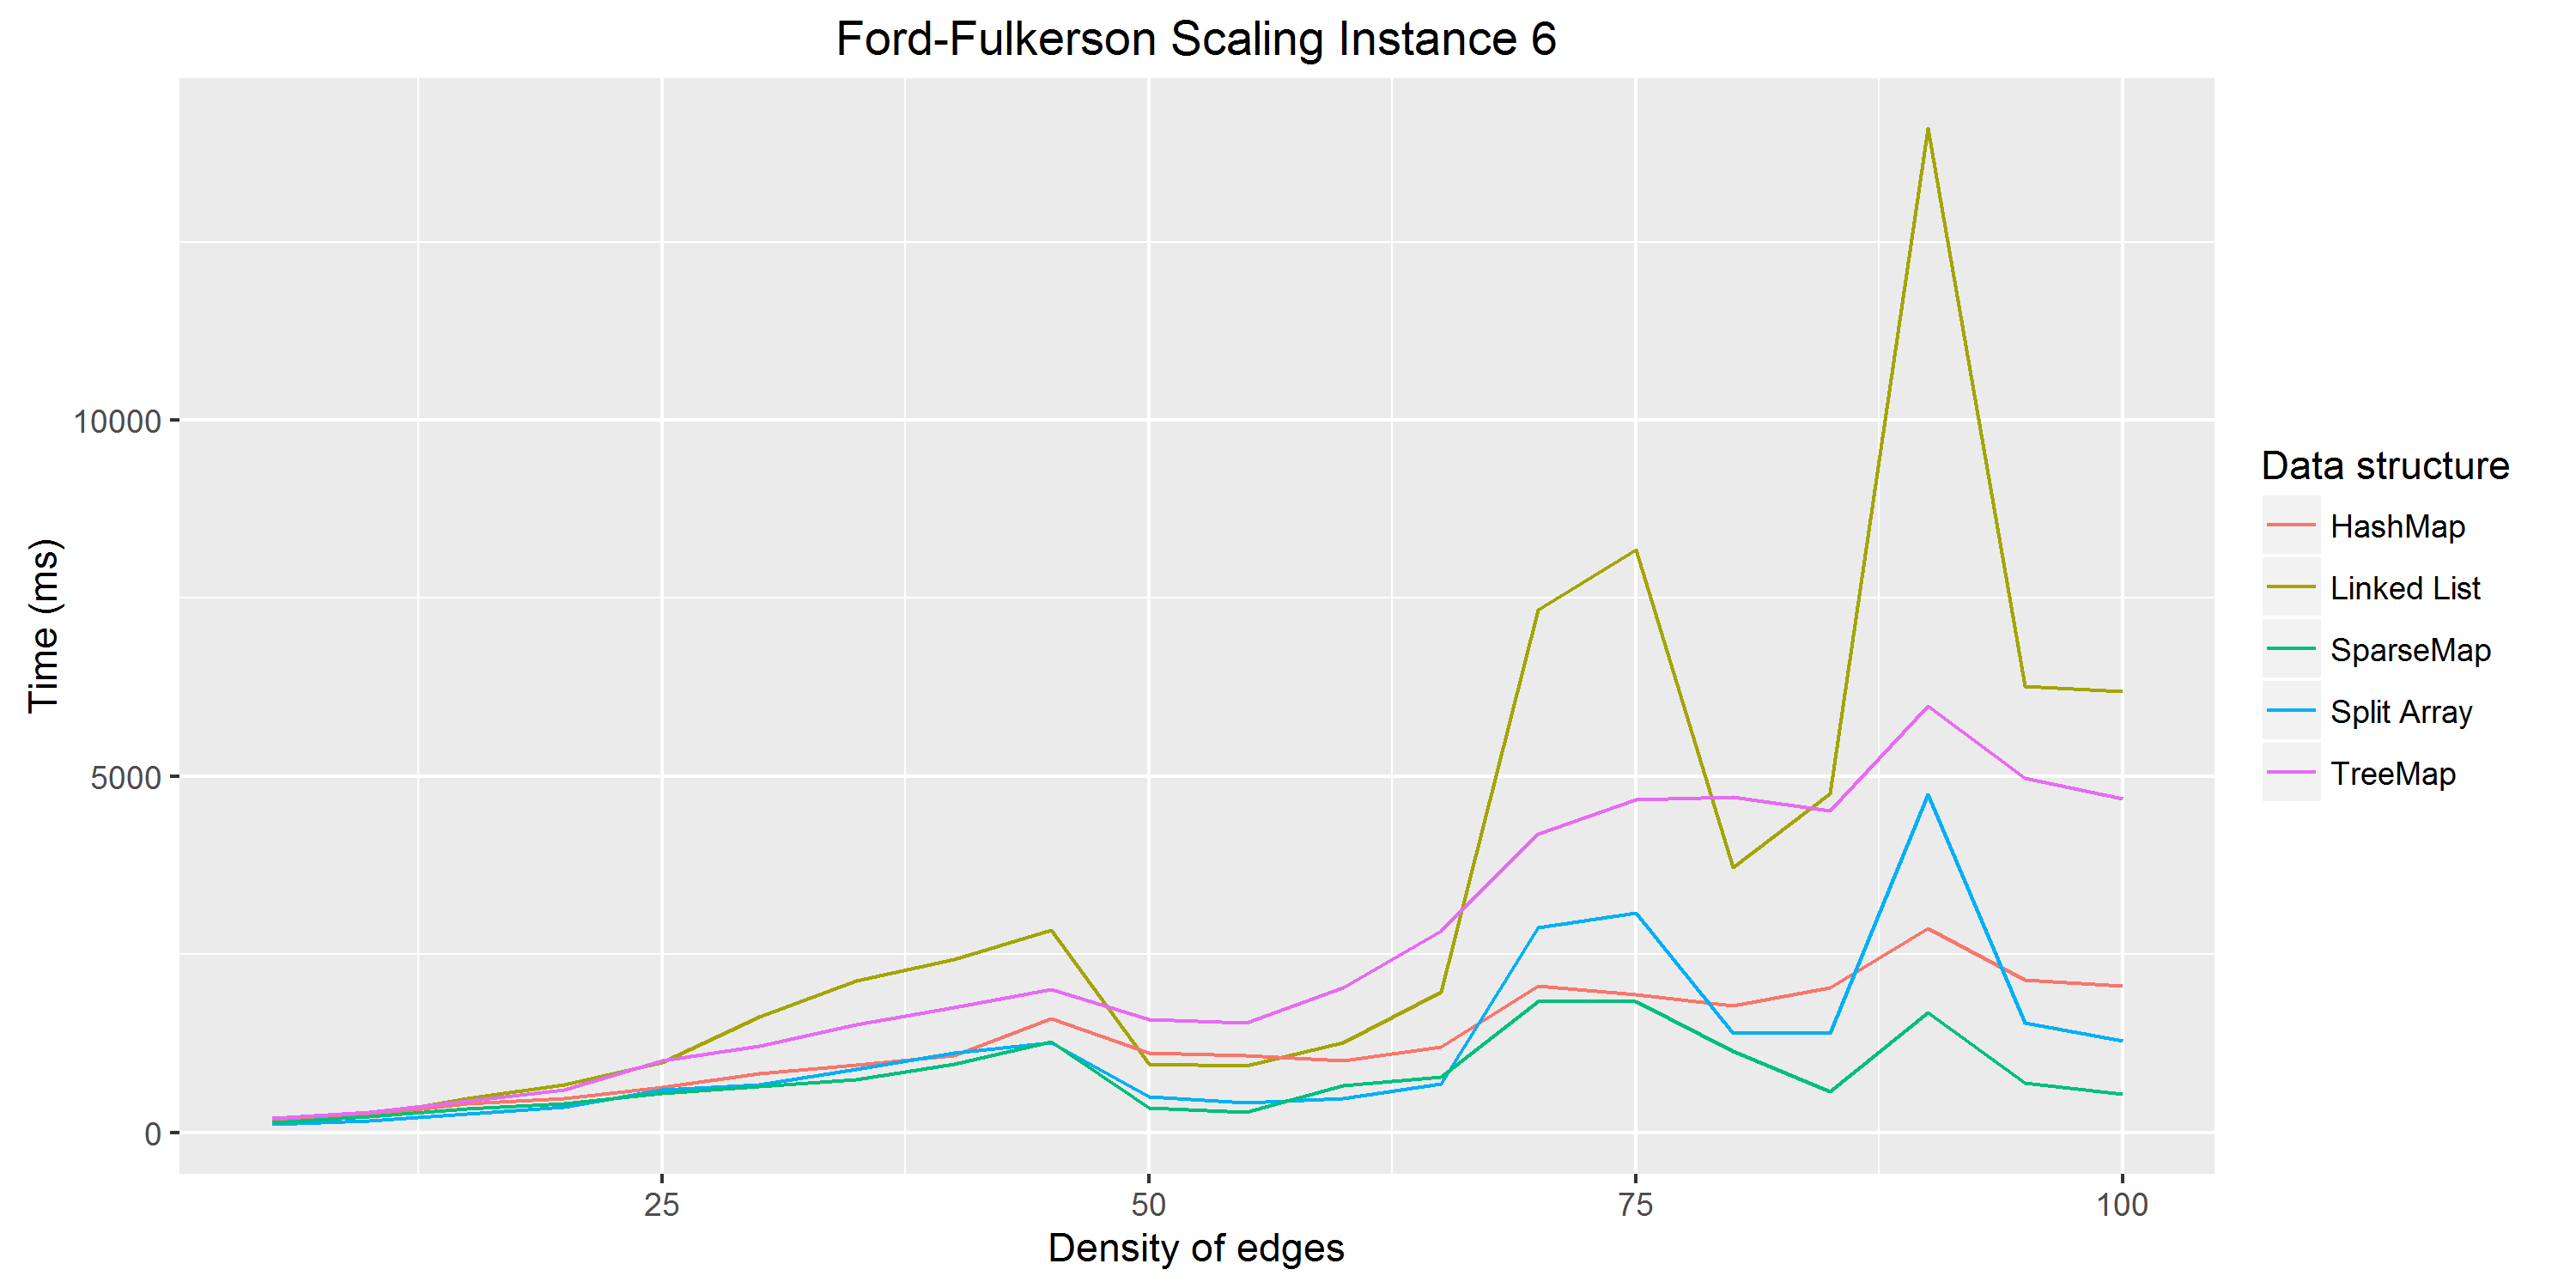
\includegraphics[scale=0.63]{images/FF6.png}
\caption{Run time of Ford-Fulkerson scaling on the instance 6.}
\label{fig:FF6}
\end{figure}

The Figure~\ref{fig:FFmean} represents the run time on each instance, with the SparseMap. Although less regular than Edmonds-Karp, Ford-Fulkerson with scaling remains stable with a run time ranging from 500 to 2500 ms to solve the maximum flow problem on complete graphs with $|V|=1000$.

\begin{figure}[H]
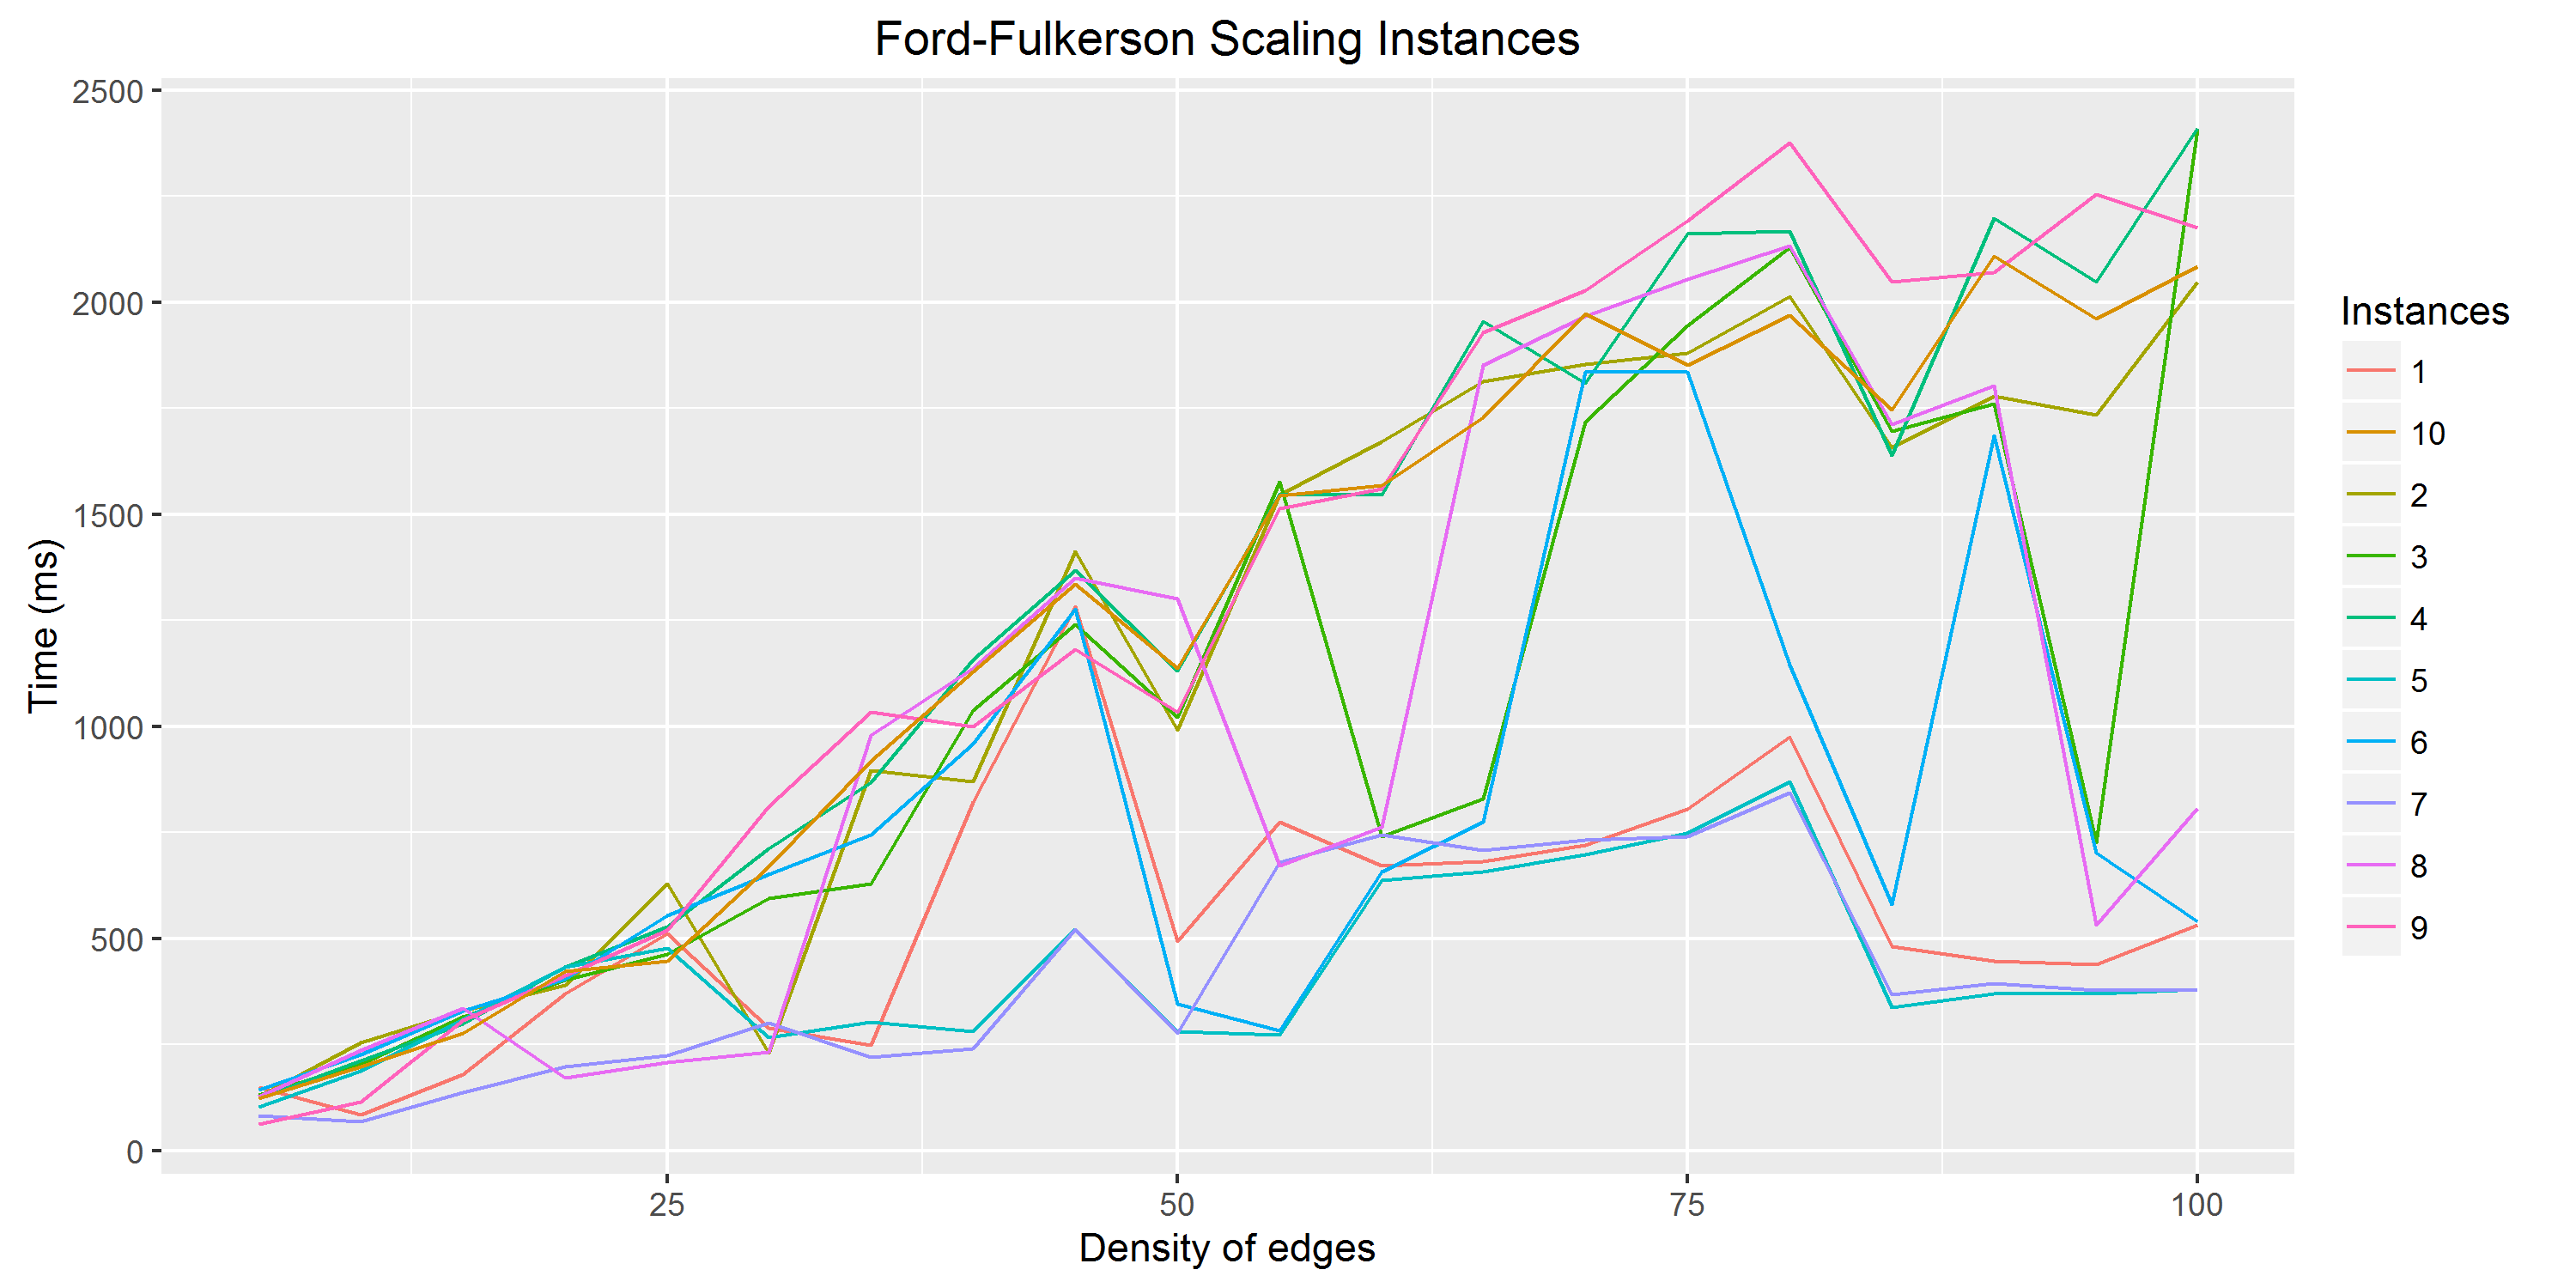
\includegraphics[scale=0.65]{images/FFmean.png}
\caption{Run time of Ford-Fulkerson scaling on all instances.}
\label{fig:FFmean}
\end{figure}

\subsubsection{Push-Relabel}
When we look at the results of the Push-Relabel, an observation is quite obvious : it is not regular at all. As shown in Figure~\ref{fig:PR6} and Figure~\ref{fig:PR8}, the run time on one instance can vary from less than 100 ms to more than 15000 ms.

\begin{figure}[H]
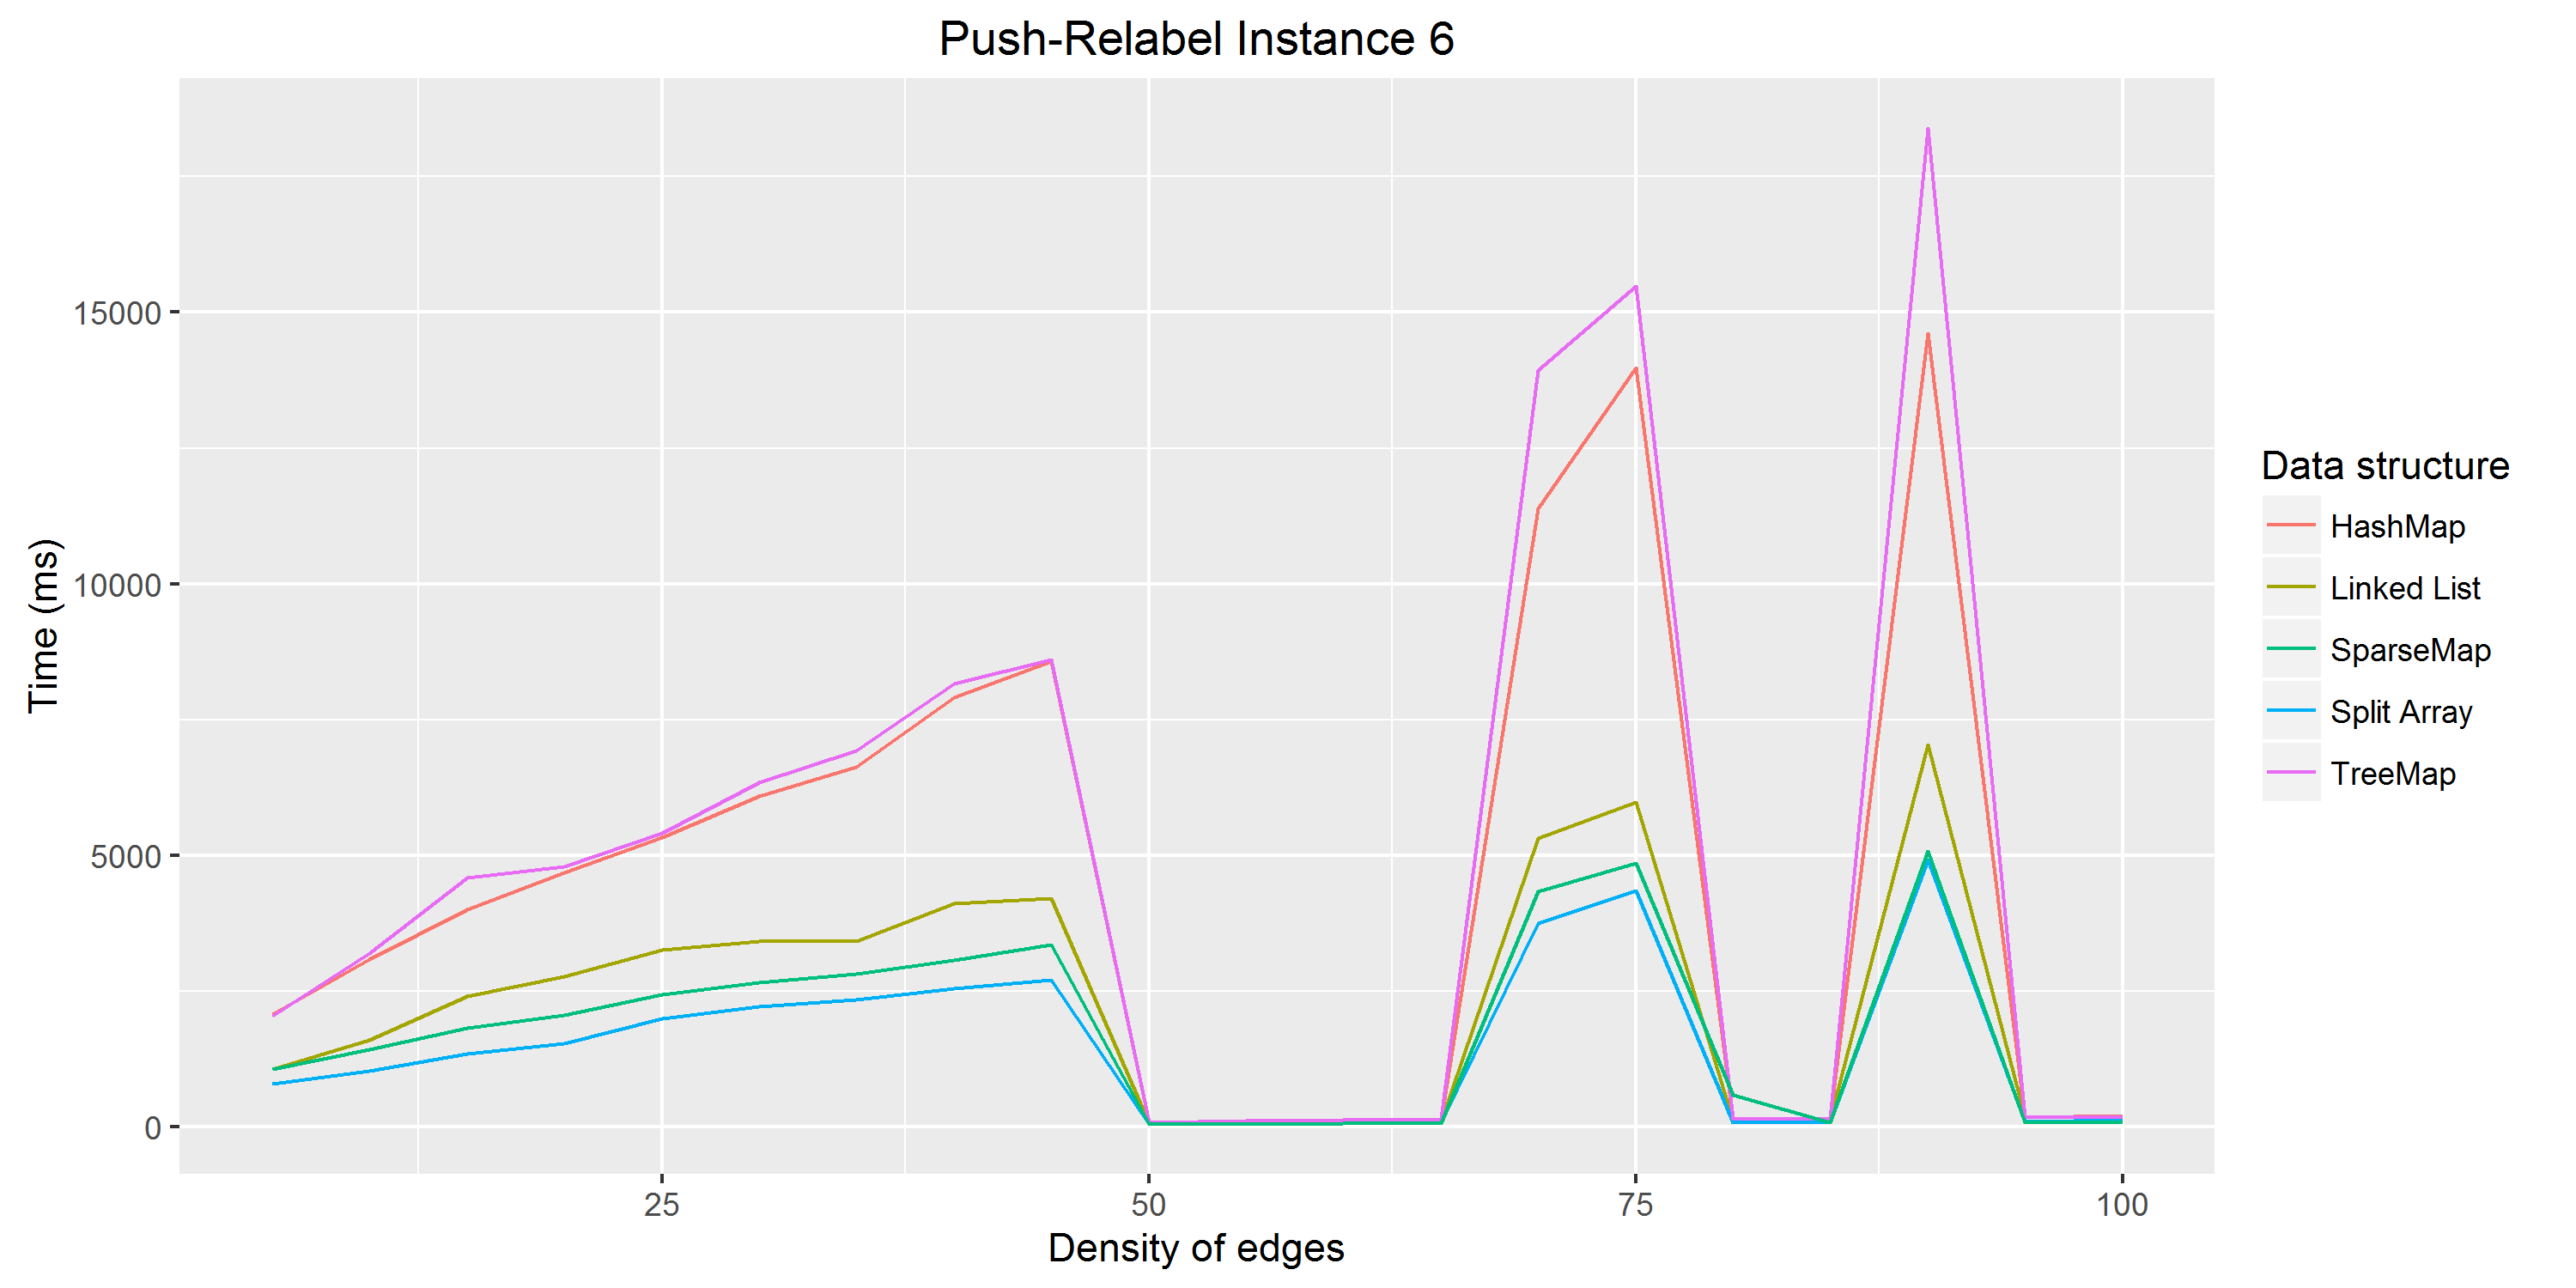
\includegraphics[scale=0.63]{images/PR6.png}
\caption{Run time of Push-Relabel on the instance 6.}
\label{fig:PR6}
\end{figure}
\begin{figure}[H]
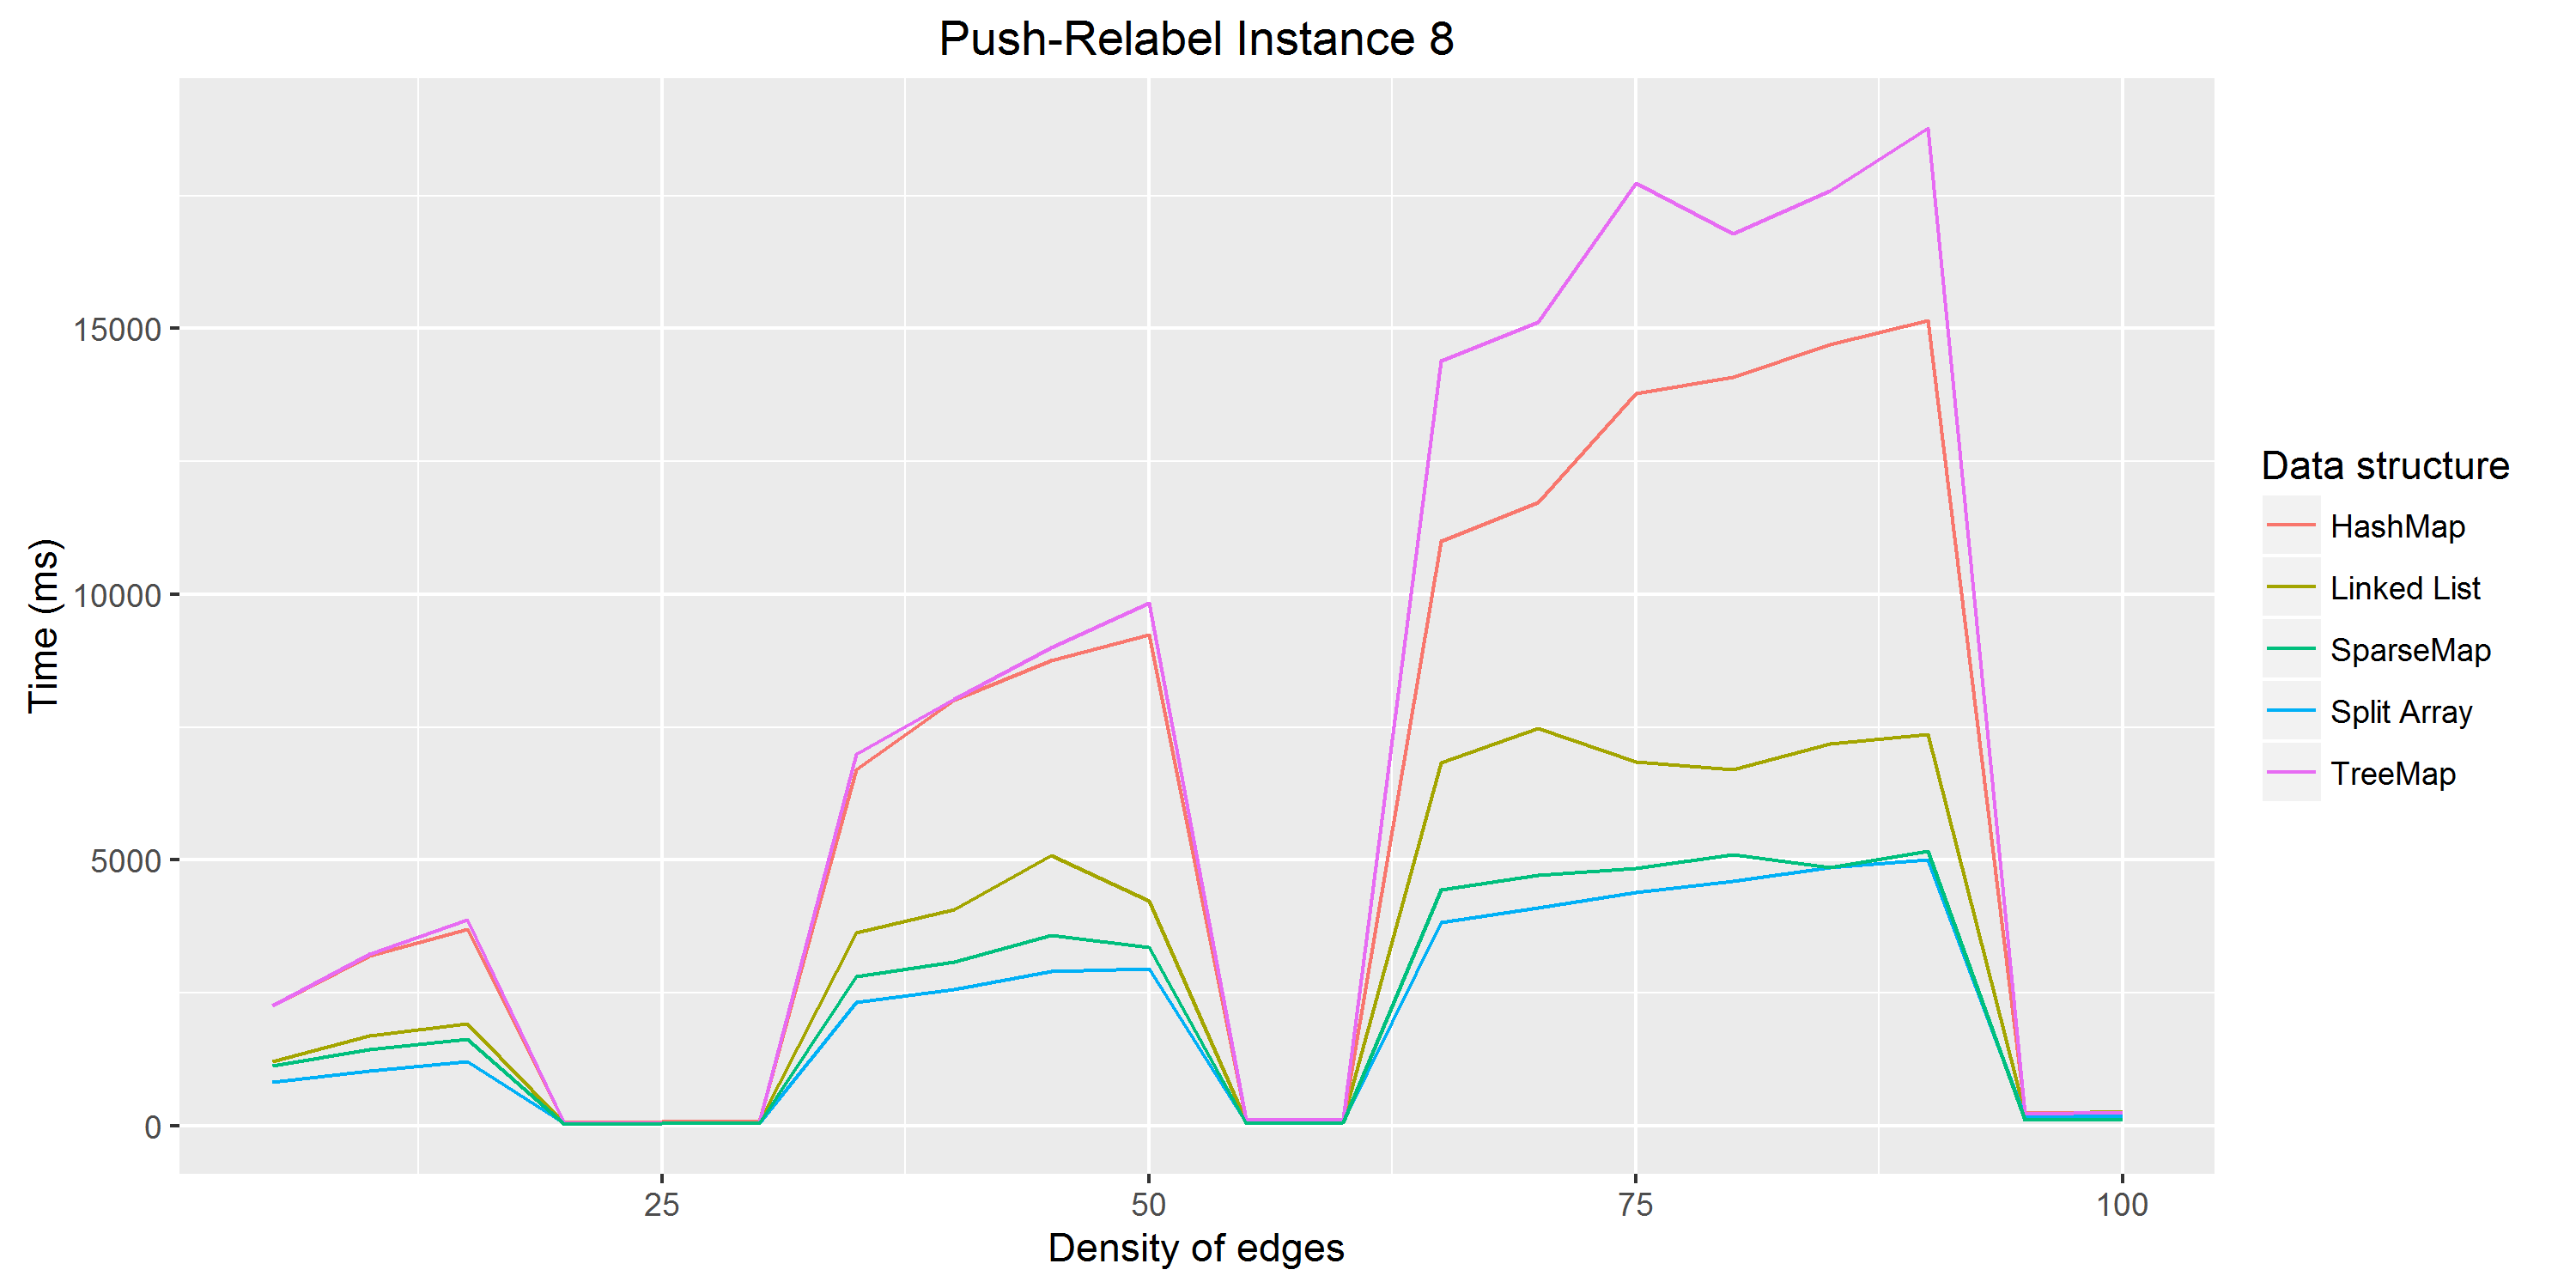
\includegraphics[scale=0.63]{images/PR8.png}
\caption{Run time of Push-Relabel on the instance 8.}
\label{fig:PR8}
\end{figure}

It may nevertheless have a stable run time but once very high and once extremely low. That is what we can observe in Figure~\ref{fig:PR10} and Figure~\ref{fig:PR7}.

\begin{figure}[H]
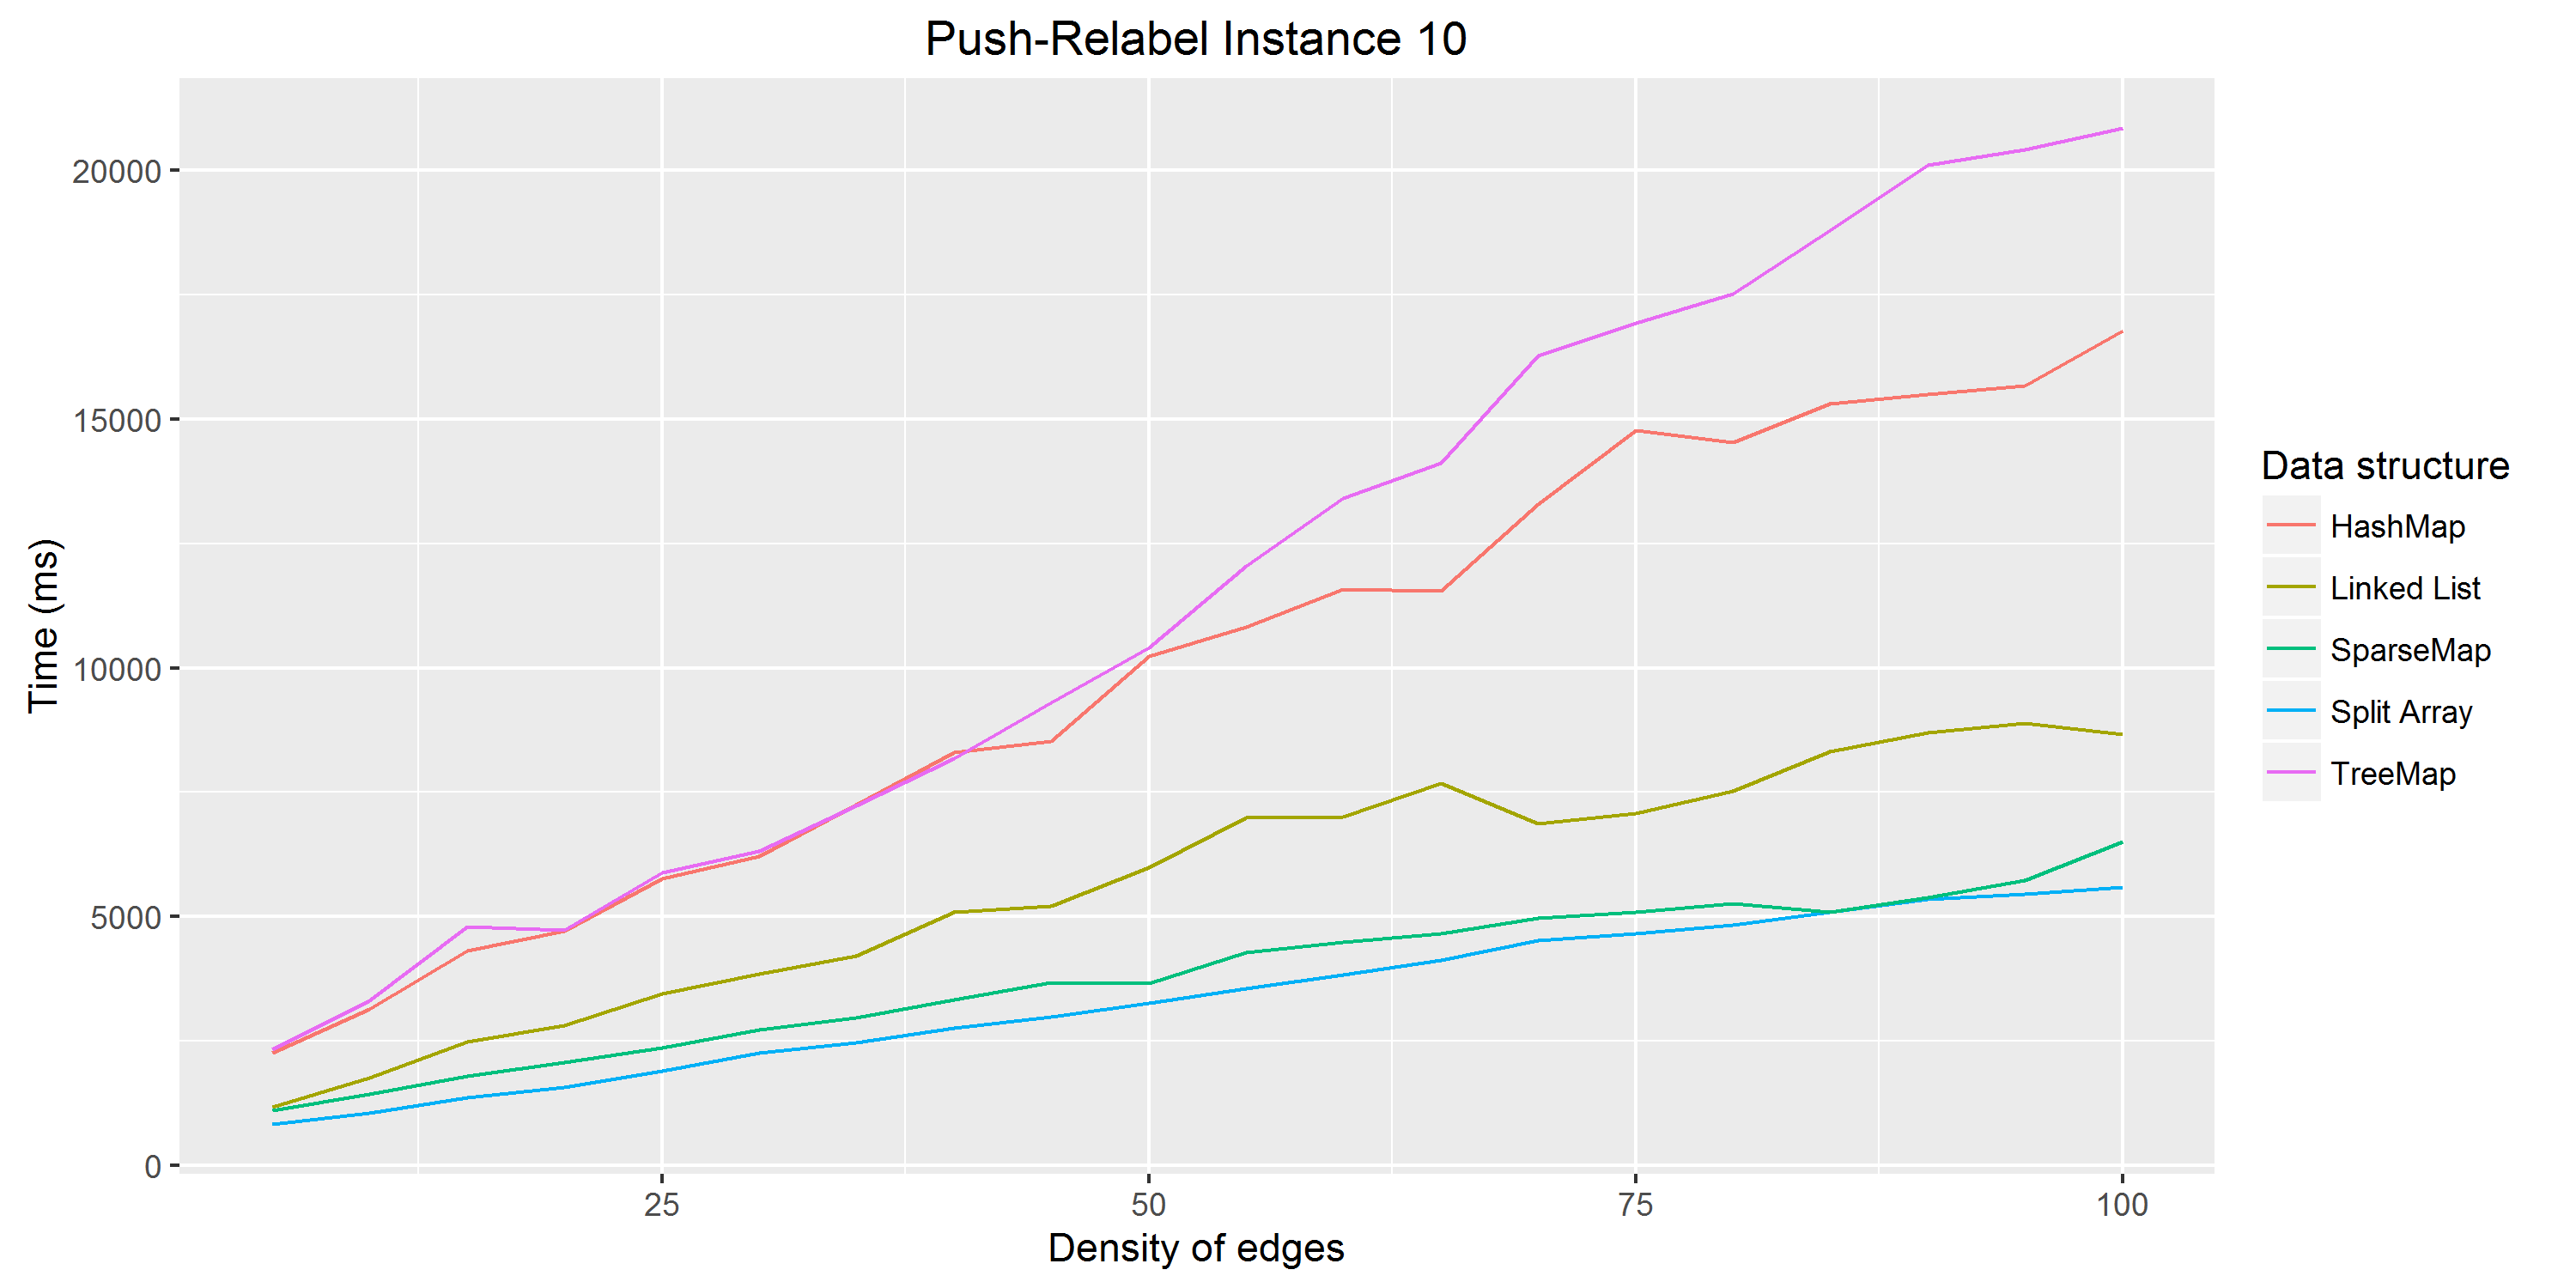
\includegraphics[scale=0.63]{images/PR10.png}
\caption{Run time of Push-Relabel on the instance 10.}
\label{fig:PR10}
\end{figure}
\begin{figure}[H]
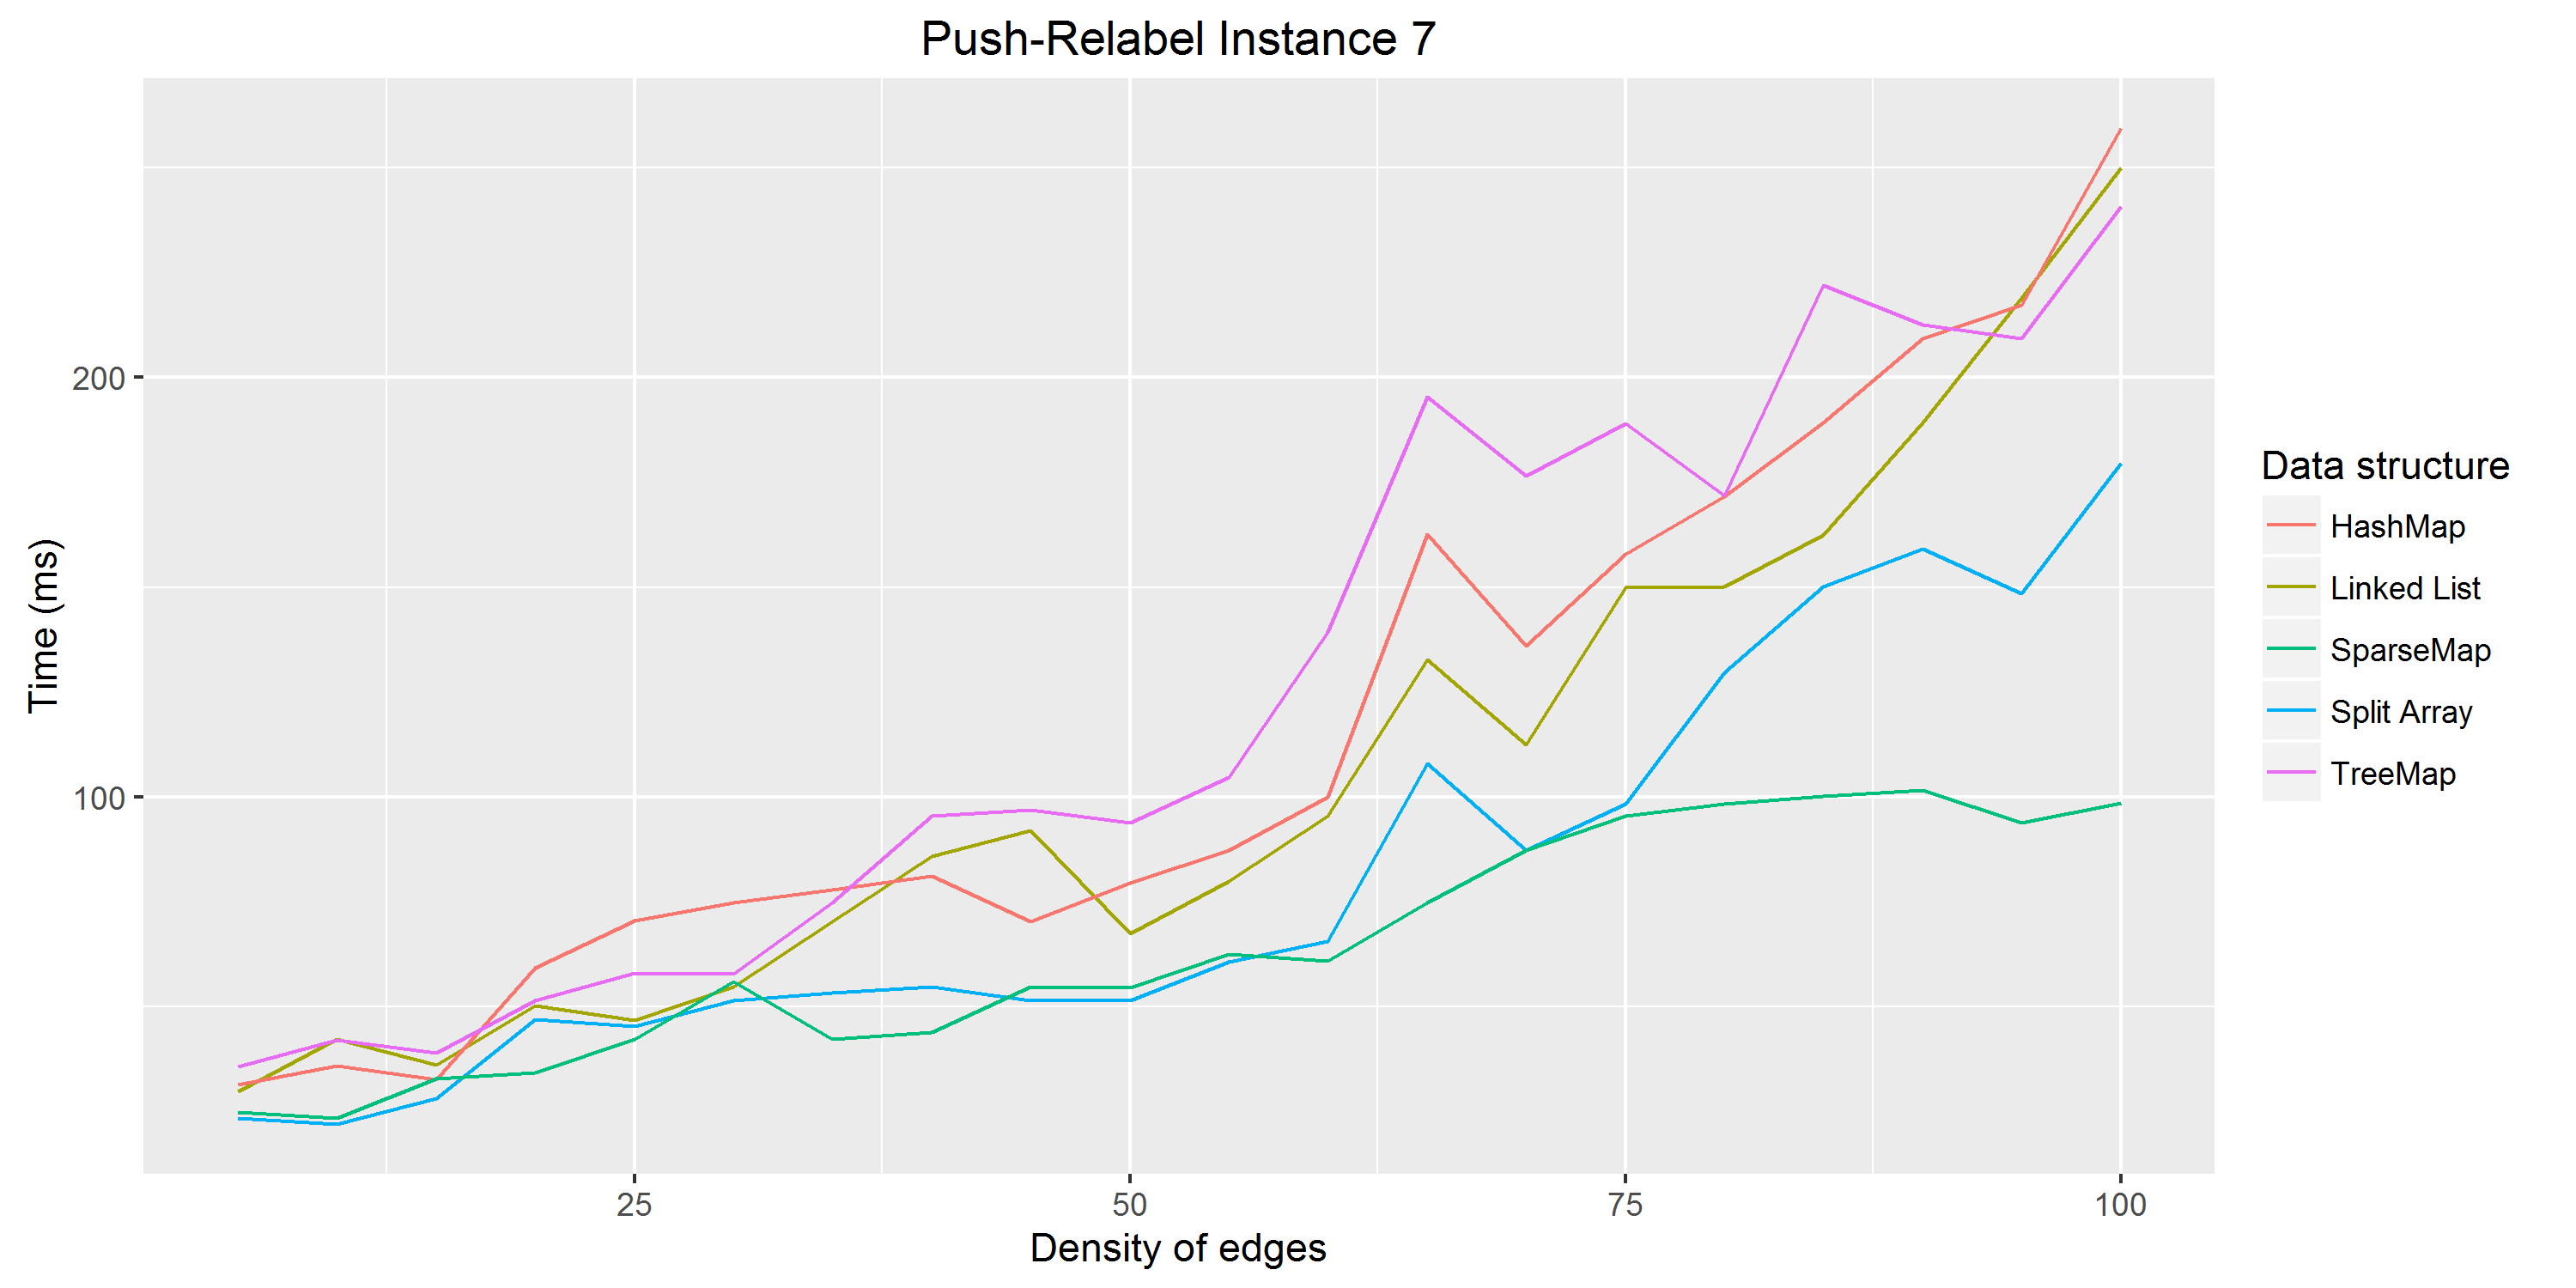
\includegraphics[scale=0.63]{images/PR7.png}
\caption{Run time of Push-Relabel on the instance 7.}
\label{fig:PR7}
\end{figure}

In terms of data structures, we notice that the HashMap and the TreeMap offer very poor performances compared to data structures based on the SparseSet. The most adapted data structure being the Split Array.

\begin{figure}[H]
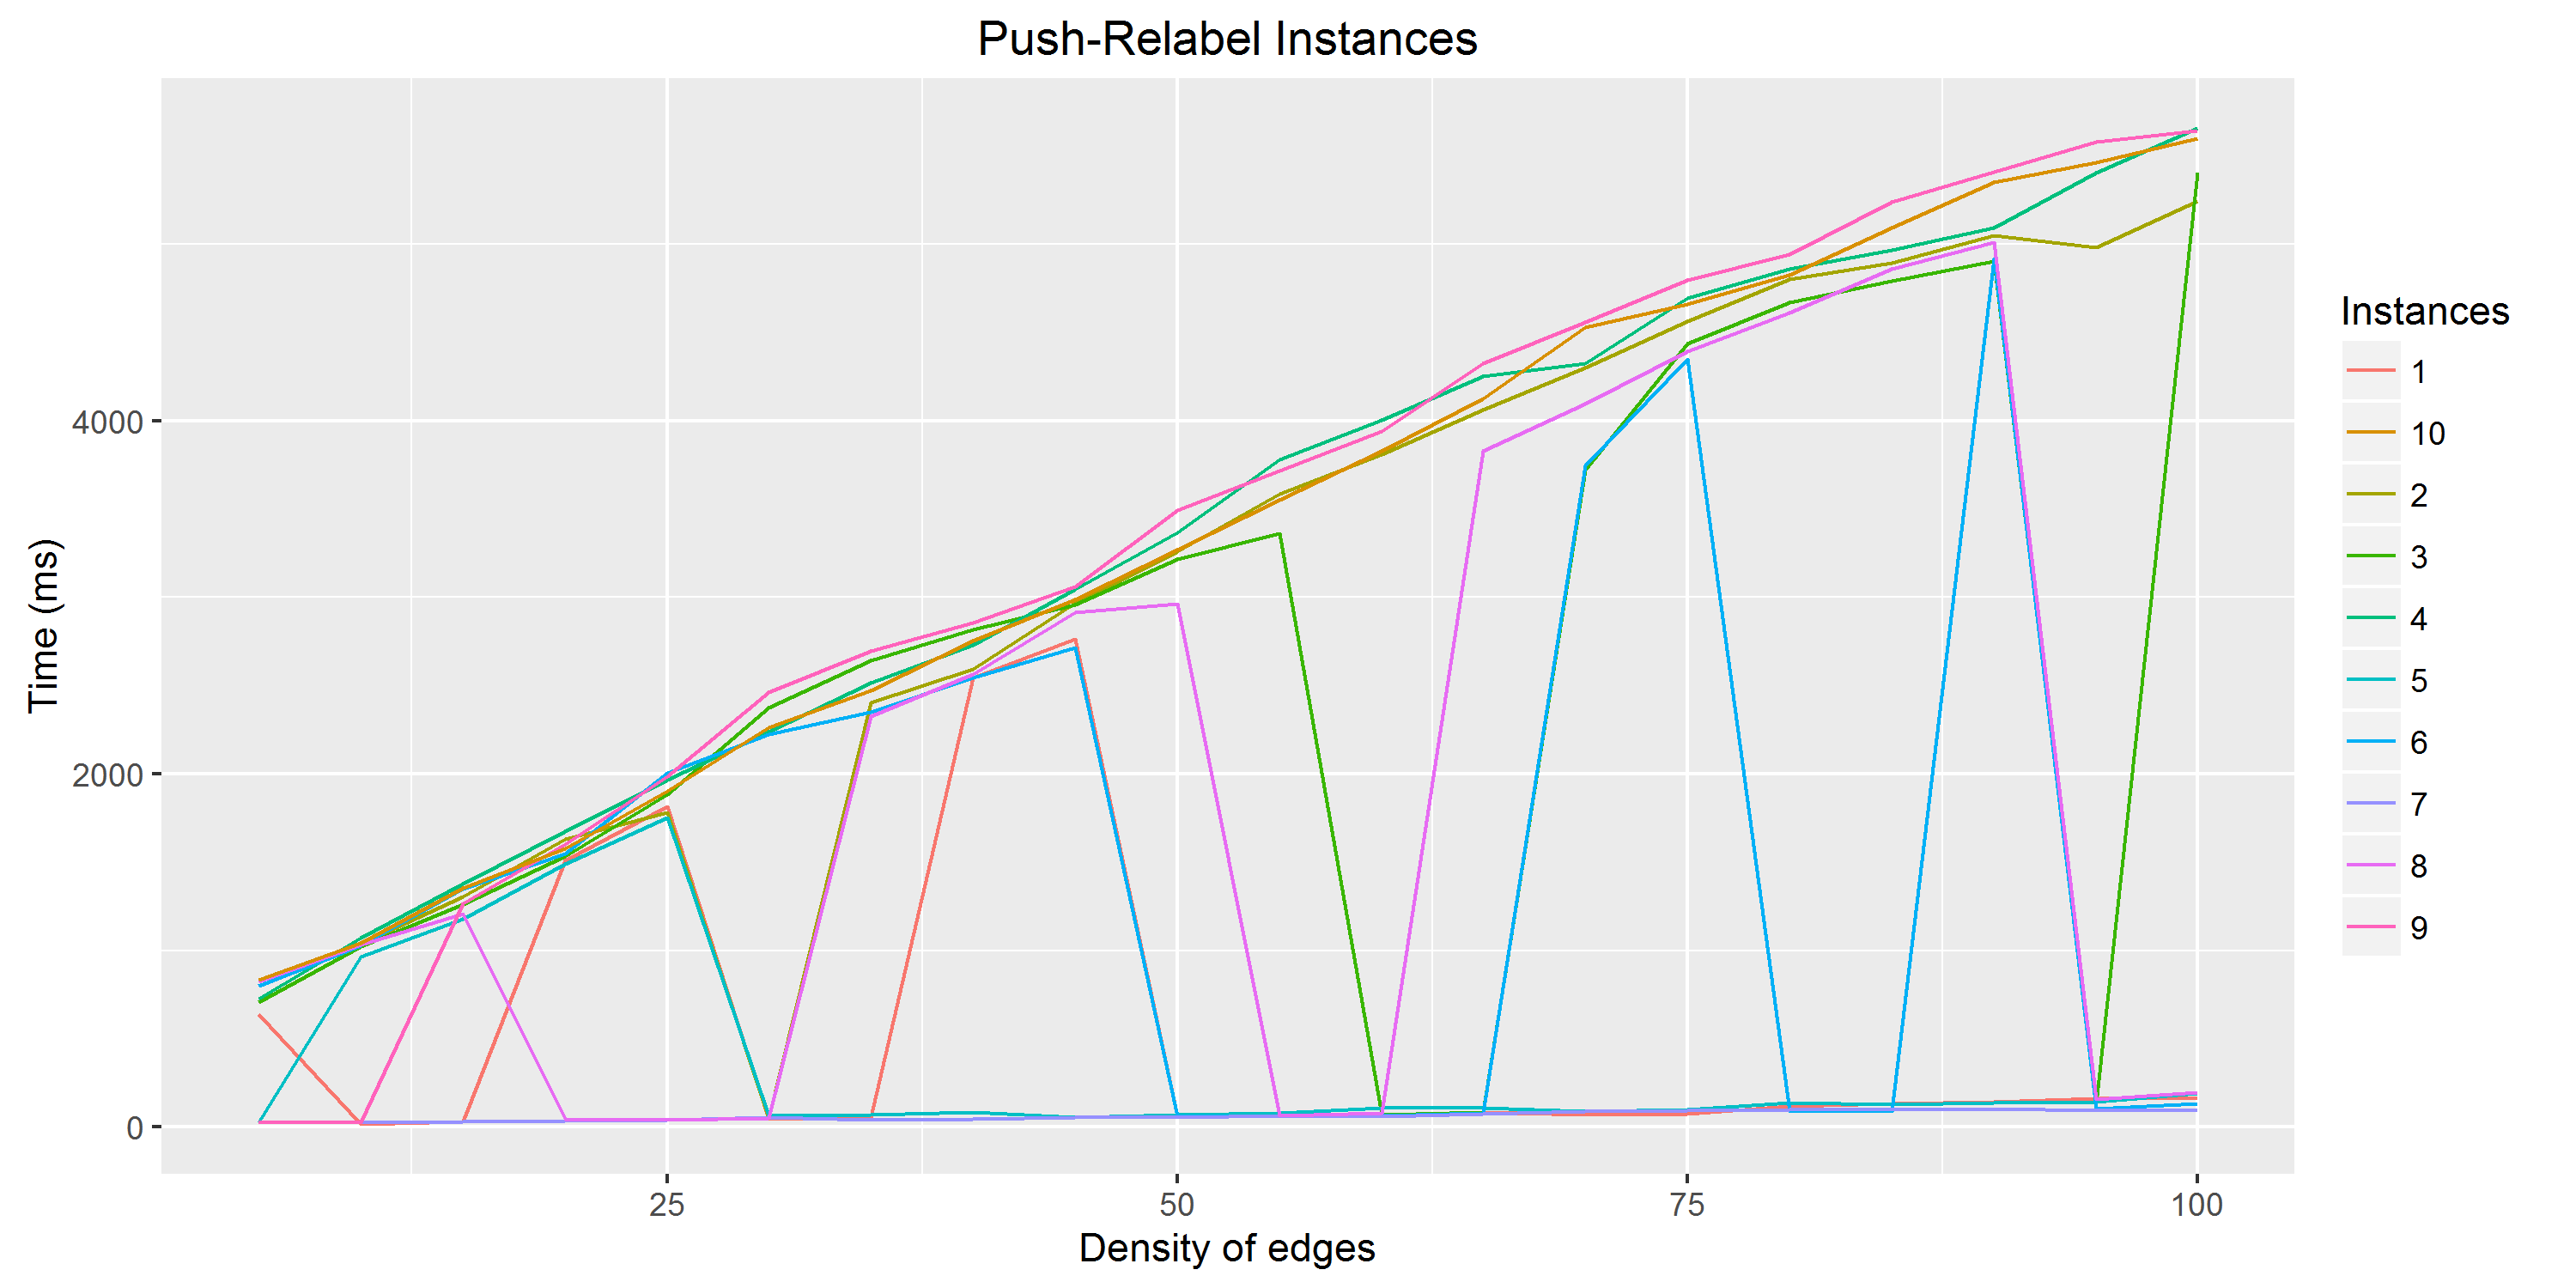
\includegraphics[scale=0.63]{images/PRmean.png}
\caption{Run time of Push-Relabel on all instances.}
\label{fig:PRmean}
\end{figure}

When displaying the run time of each instance with its best data structure, we obtain a very disparate graph, as we can see in Figure~\ref{fig:PRmean}. Indeed, the Push-Relabel solve the maximum flow problem on complete graphs with $|V|=1000$ with a run time ranging from 100 ms to 5500 ms.

\subsubsection{Comparison}
The Figure~\ref{fig:MeanInstances} represents, for each algorithm, the average run time on all instances with its best data structure. The performances are close but Edmonds-Karp with the Split Array is the most appropriate algorithm to solve the maximum flow problem with graphs having a high-density of edges.

\begin{figure}[H]
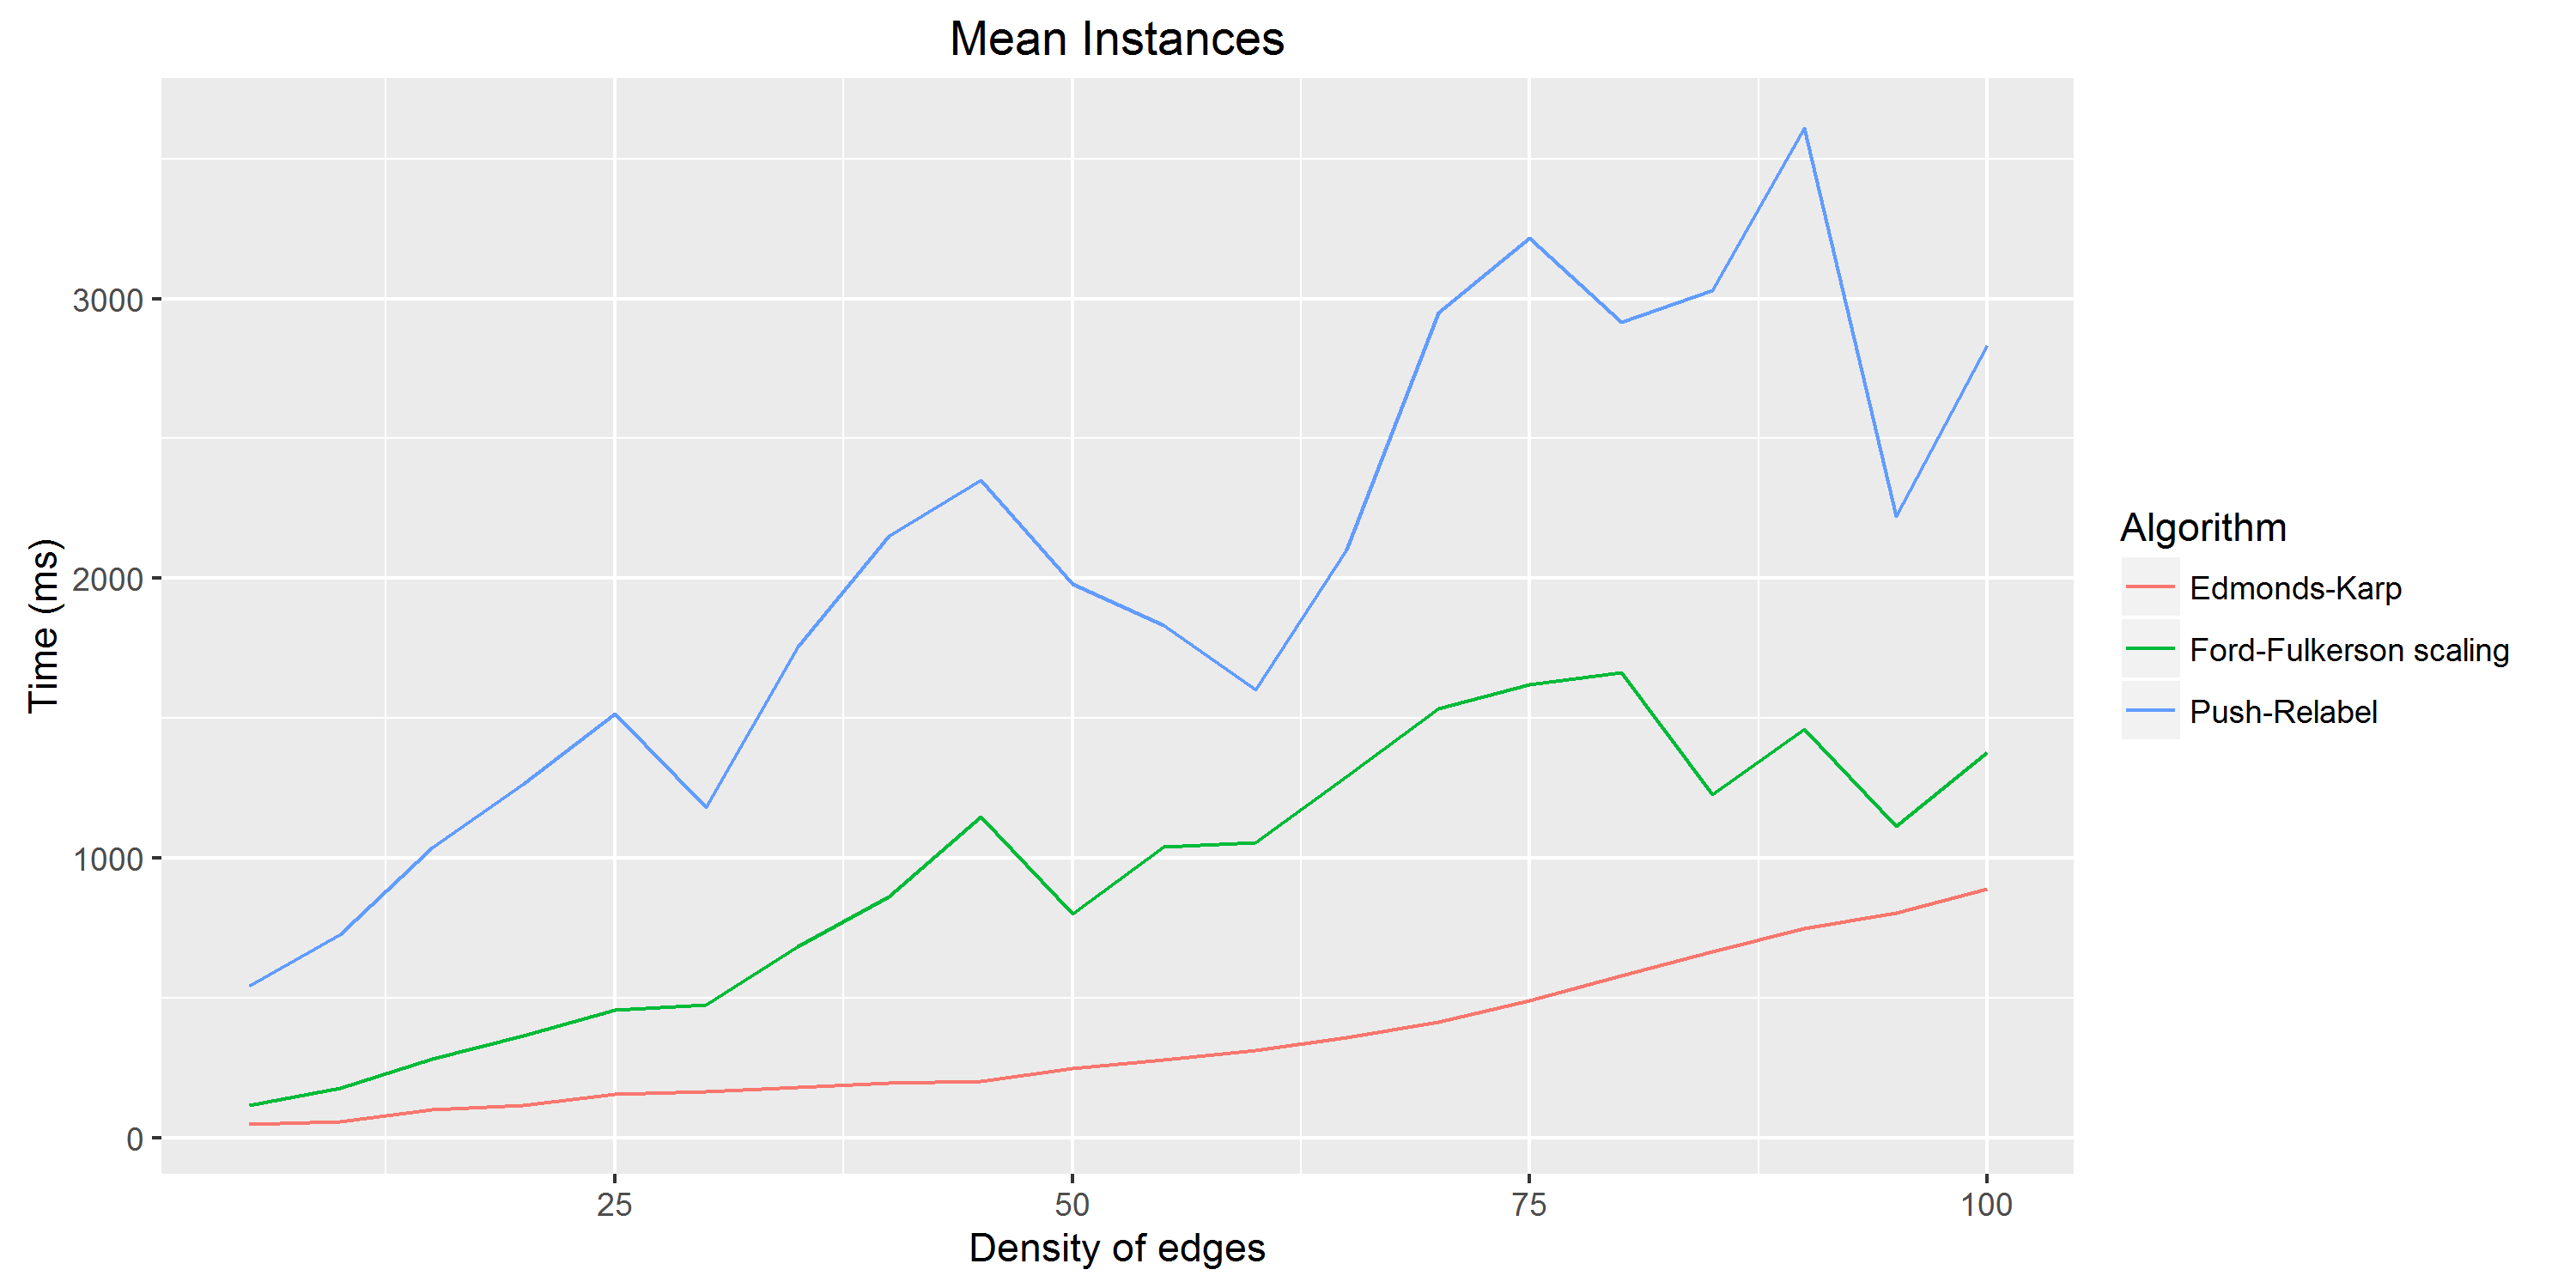
\includegraphics[scale=0.65]{images/MeanInstances.png}
\caption{Average run time of the three algorithms on all instances.}
\label{fig:MeanInstances}
\end{figure}

\subsection{Size variation instances}
Graphes + grosse grosse explication

\section{Analysis}

J'explique quel algo est meilleur avec quel type de graphe et je tire des conclusions.

Faut mettre le profiler quelque part aussi